\documentclass[aspectratio=169]{beamer}
\usetheme{Darmstadt}
\usepackage[T1,T2A]{fontenc}
\usepackage[utf8]{inputenc}
\usepackage[english]{babel}
\usepackage{amsmath,amssymb}
\usepackage{mathtext}
\usepackage{amsthm}
\usepackage{graphicx}
\usepackage{cmap}
\usepackage{bbm}
\usepackage{tikz}
\usepackage{float}


\usepackage[backend=biber,style=alphabetic,sorting=ynt]{biblatex}
\usepackage{csquotes}
\addbibresource{bibliography.bib}

\usepackage{graphicx}

% Types


\newcommand{\hm}[1]{#1\nobreak\discretionary{}{\hbox{\ensuremath{#1}}}{}}

\DeclareMathOperator{\sgn}{sign}
\DeclareMathOperator*{\var}{var}   
\DeclareMathOperator*{\cov}{cov}

\newcommand{\1}{\mathbbm{1}} 
\newcommand{\R}{\mathbb{R}}
\newcommand{\N}{\mathbb{N}}
\renewcommand{\P}{P}
\newcommand{\eps}{\varepsilon}

\newcommand\cA{{\cal A}}
\newcommand\cE{{\cal E}}
\newcommand\cC{{\cal C}}
\newcommand\cF{{\cal F}}
\newcommand\cG{{\cal G}}
\newcommand\cK{{\cal K}}
\newcommand\cL{{\cal L}}
\newcommand\cB{{\cal B}}
\newcommand\cN{{\cal N}}
\newcommand\cM{{\cal M}}
\newcommand\cX{{\cal X}}
\newcommand\cD{{\cal D}}
\newcommand\cR{{\cal R}}
\newcommand\cP{{\cal P}}
\newcommand\cQ{{\cal Q}}
\newcommand\cS{{\cal S}}
\newcommand\cT{{\cal T}}
\newcommand\cV{{\cal V}}
\newcommand\cZ{{\cal Z}}

\newcommand{\wt}{\widetilde}

\AtBeginSection[]
{
  \begin{frame}
    \frametitle{Table of Contents}
    \tableofcontents[currentsection]
  \end{frame}
}
\title{'Pricing under Rough Volatilty Models' Lab Report}
\author{Artemy Sazonov}
\date{July 1, 2022}
\institute{Lomonosov Moscow State University}

\begin{document}
    \maketitle

    \section{General theory}
        \subsection{Realized volatility}
            \begin{frame}{Realized volatility - I}
                Consider a stochastic volatility model 
                \begin{equation}\label{model:SVM}
                    dS_t = \mu_t S_t dt + \sigma_t S_tdW_t,
                \end{equation}
                where $S_t$ is an asset price process, and $\sigma_t$ is a stochastic volatility process representing a so-called \emph{spot volatility}.
                \begin{definition}
                    The \emph{realized volatility} of a price process $S$ over time interval $[t, t + \delta]$ sampled along the time partition $\pi^n$
                    is defined as 
                    \begin{equation}\label{def:RV}
                        RV_{t, t + \delta}(\pi^n) = \sqrt{\sum_{\pi^n \cap [t, t + \delta]} \left(\log S_{t^n_{i+1}} - \log S_{t^n_{i}}\right)^2}.
                    \end{equation}
                \end{definition}
            \end{frame}

            \begin{frame}{Realized volatility - II}
                \begin{definition}
                    Let $S$ satisfy \eqref{model:SVM}. Then the integrated variance is defined as
                    \begin{equation}\label{def:IV}
                        IVar_t = \int_{0}^{t} \sigma_s^2 ds.
                    \end{equation}
                \end{definition}

                \begin{theorem} 
                    As time partition scale and $\delta$ tend to $0$, \begin{equation}
                        \frac{RV_{t, t + \delta}}{\sqrt{\delta}} \overset{\mathbb{P}}{\to} \sigma_t
                    \end{equation}
                \end{theorem}
            \end{frame}   
        \subsection{Fractional stochastic processes}
            \begin{frame}{Fractional stochastic processes - I}
                \begin{definition}
                    The \emph{fractional Brownian motion} $(W_t^H)_{t\in \mathbb{R_+}}$ with Hurst 
                    parameter $H \in (0, 1)$ is a Gaussian process with the following properties:
                    \begin{enumerate}
                        \item $W_0^H = 0$,
                        \item $\mathbb{E}\left[W_t^H\right] \equiv 0$,
                        \item $\mathbb{E}\left[W_s^H W_t^H\right] = \frac{1}{2} \left(t^{2H} + s^{2H} - |t-s|^{2H}\right)$.
                    \end{enumerate}
                \end{definition}
            \end{frame}   

            \begin{frame}{Fractional stochastic processes - II}
                \begin{definition}
                    A stationary fOU process $X_t$ is defined as the stationary solution of the stochastic differential equation
                    \begin{equation}
                        dX_t = \nu dW^H_t - \alpha (X_t - m)dt,
                    \end{equation}
                    where $m \in \mathbb{R}$ and $\nu$ and $\alpha$ are positive parameters.
                \end{definition}
            \end{frame} 
        \subsection{Long memory of processes}
            \begin{frame}{Long memory of processes}
                \begin{definition}
                    A process $X_t$ is said to have a long memory, if 
                    \begin{equation}
                        \sum_{k=0}^{\infty}\cov\left[X_1 , X_{k} - X_{k-1}\right] = \infty.
                    \end{equation}
                \end{definition}
        
                In particular, the fractional Brownian motion with $H > \frac{1}{2}$ is a long-memory process.
                Long-memory of the stochastic volatility process in stochastic volatilty models framework used to be a 
                widely-accepted stylized fact.
            \end{frame}

    \section{Rough fractional stochastic volatility model}
        \subsection{Definitions}
            \begin{frame}{RFSV - I}
                Let there be a riskless asset $B_t \equiv 1$, and a risky asset, whose price $S_t$ is defined 
                by the following equations: 
                \begin{align}
                    & dS_t          = \alpha S_t dt + \sigma_t S_tdW_t,               \label{model:RFSVasset} \\
                    & d\log\sigma_t = \alpha (m - \log\sigma_t) dt + \nu dW_t^H.      \label{model:RFSVvol}
                \end{align}
                As a stylized fact we shall demand the stationarity of log-increments.
            \end{frame}

            \begin{frame}{RFSV - II}
                Let $m(q, \Delta, \pi^n)$ be a sample $q$-th absolute moment of $\log RV_{t+\Delta} - \log RV_t$:
                \begin{equation}
                    m(q, \Delta, \pi^n) := \frac{1}{n} \sum_{t} \left|\log RV_{t + \Delta} - \log RV_t\right|^q,
                \end{equation}
                i.e. $m(q, \Delta, \pi^n)$ is an empirical counterpart of $\mathbb{E}\left[\left|\log RV_{\Delta} - \log RV_0\right|^q\right]$.
                In this work we shall use the uniform partition of time scale with each step being equal to $15$ minutes, so we omit the $\pi^n$ notation and use $m(q, \Delta)$.
                Via the explicit formula for the covariance function of the log-volatility in the RFSV model, we can write 
                a closed-form expression for a theoretical $m(2, \Delta)$:
                \begin{equation}
                    m(2, \Delta) = 2\left(\var \log\sigma_{t} - \cov\left[\log\sigma_{t}, \log\sigma_{t+\Delta}\right]\right).
                \end{equation}
            \end{frame}

        \subsection{Estimation}
            \begin{frame}{}
                In the present paper we used high-frequency data for the three types of assets:
                \begin{enumerate}
                    \item\textbf{Stocks}: Yandex, Sberbank, Gazprom, VTB, Moscow Exchange, Lukoil, and X5 Group;
                    \item\textbf{Depositary reciepts}: Sberbank, Gazprom, VTB, and Lukoil;
                    \item\textbf{Funds}: AEX, AORD, BFX, BVSP, DJI, FCHI, FTMIB, FTSE, GDAXI, GSPTSE, HSI, IBEX, IXIC, KS11, KSE, MXX, N225, OMXC20, OMXHPI, OMXSPI, OSEAX, RUT, SMSI, SPX, SSEC, SSMI.
                \end{enumerate}
            \end{frame}

            \begin{frame}
                \begin{figure}[htbp]
                    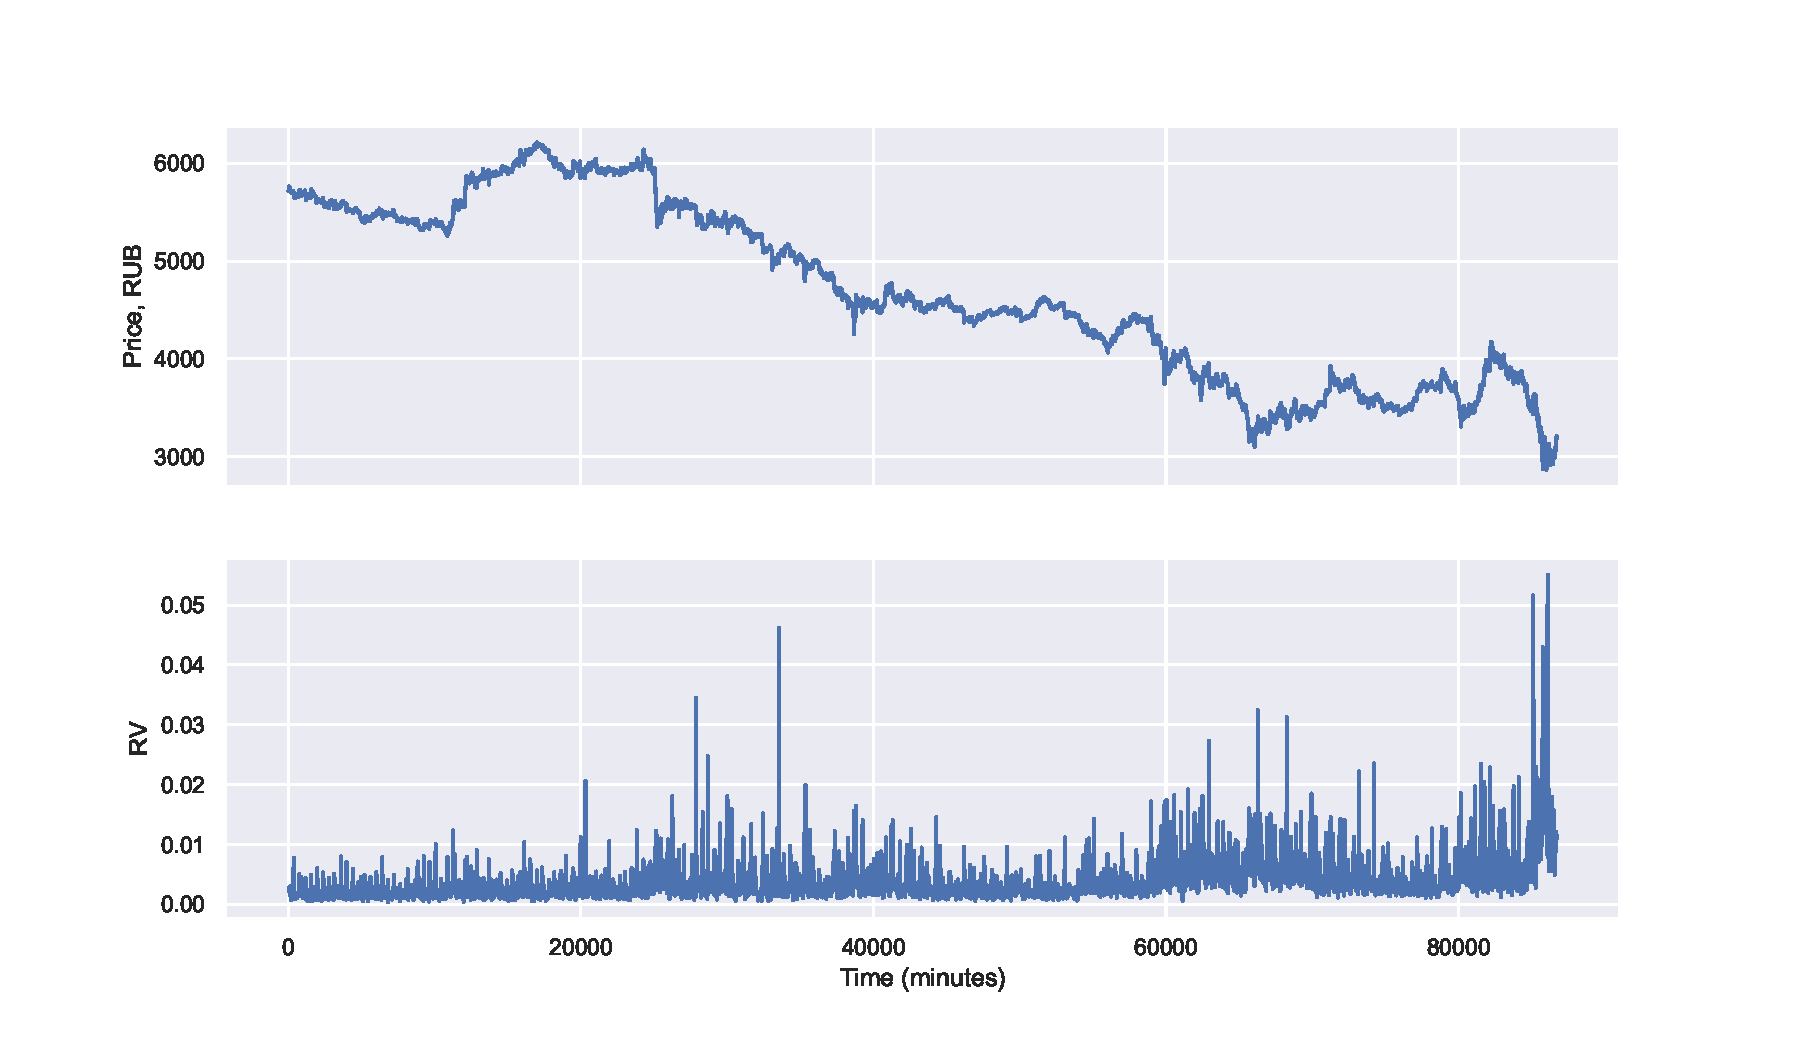
\includegraphics[width=0.75\linewidth]{fig/YNDX RX Equity RVol.pdf}
                    \caption{YNDX RX Equity. Price and Realized Volatility}
                    \label{fig:priceRV} 
                \end{figure}
            \end{frame}

            \begin{frame}{Main assumption}
                \textbf{Main assumption}: for some $s_q > 0 $, $b_q > 0$ and $N = \left[\frac{T}{\Delta}\right]$ 
                (number of RV estimations via disjoint windows)
                \begin{equation}\label{eq:mainassumpt}
                    N^{qs_q} m(q, \Delta) \xrightarrow[\Delta \to 0+]{} b_q.
                \end{equation}
                Under additional technical conditions, equation \eqref{eq:mainassumpt} is equivalent to that the volatility process 
                belongs to the Besov smoothness space $B^{s_q}_{q, \infty}$ and for all $\tilde{s}_q > s_q$ does not belong to 
                $B^{\tilde{s}_q}_{q, \infty}$ (see [Ros08]).
            \end{frame}


            \begin{frame}{}
                \begin{figure}[htbp]
                    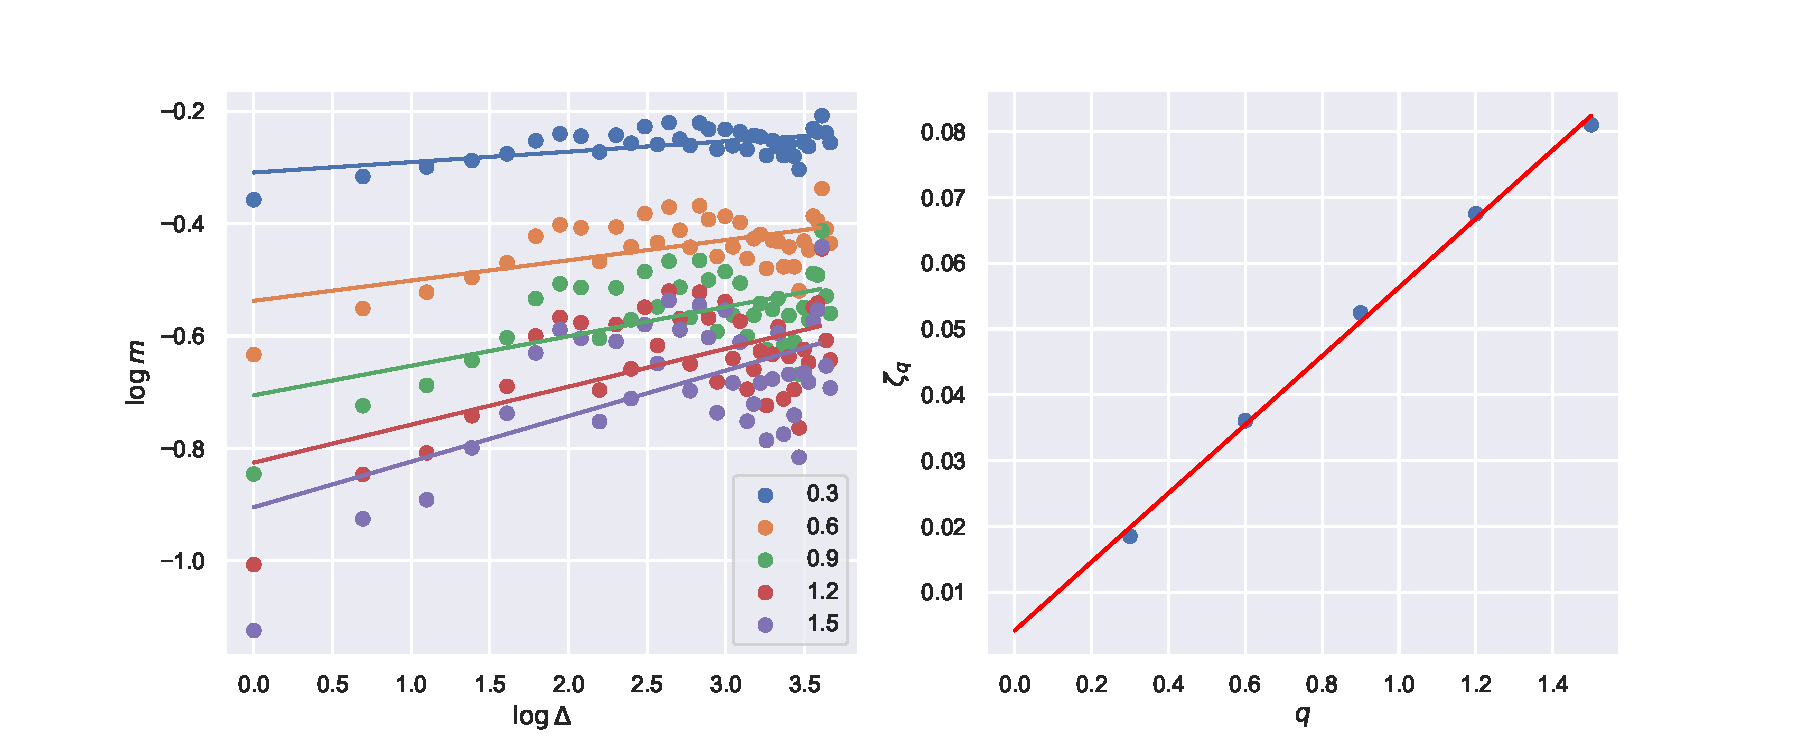
\includegraphics[width=\textwidth]{fig/YNDX RX Equity Hurst Est.pdf}
                    \caption{YNDX RX Equity. Regression-based roughness estimation}
                    \label{fig:logMDelta}
                \end{figure}
            \end{frame}

            \begin{frame}{}
                It has been shown that under stationarity assumptions and linearity of Figure \ref{fig:logMDelta} (left)
                \begin{equation}
                    \mathbb{E}\left[\left|\log\sigma_{t+\Delta} - \log\sigma_{t}\right|^q\right] = K_q \Delta^{\zeta_q},
                \end{equation} 
                and the $s_q$ does not depend on $q$. 
                We note that the graphs for $\zeta_q$ are slightly concave, which correlates with [GJR14] results.
                They conclude that this effect takes place due to the finite statistical population size. It has been proven in [GJR14] that $\log\mathbb{E}[\sigma_{t}\sigma_{t+\Delta}]$ and $\log \cov[\log\sigma_t, \log\sigma_{t+\Delta}]$ are linear in $\Delta^{2H}$. And we indeed observe this behaviour in the majority of plots (especially for $\Delta < 20$, where we have enough data to work with).
                Numerical instability occurs when $\Delta$ is too large due to the lack of HF data.
            \end{frame}

            \begin{frame}{}
                \begin{figure}
                    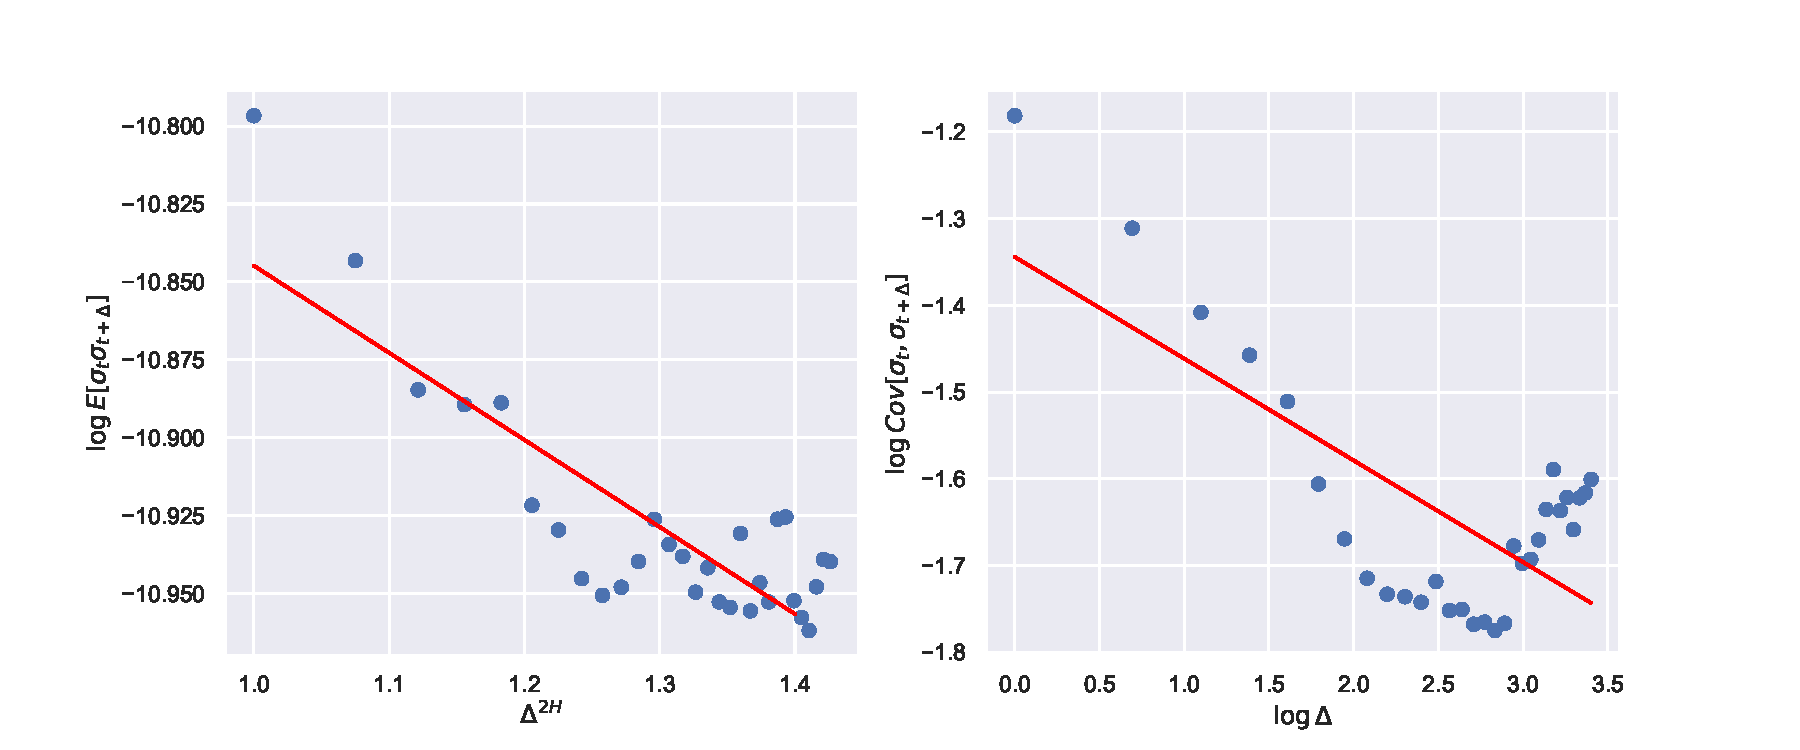
\includegraphics[width=\textwidth]{fig/YNDX RX Equity logE vs logD.pdf}
                    \caption{YNDX RX Equity. Empirical counterpart of $\log\mathbb{E} \left[\sigma_{t}\sigma_{t+\Delta}\right]$ as a function of $\Delta^{2H}$ (left) and Empirical counterpart of $\log\cov [\log\sigma_{t}, \log\sigma_{t+\Delta}]$ as a function of $\log\Delta$ (right)}
                \end{figure}
            \end{frame}

            \begin{frame}{}
                \begin{table}[htbp]
                    \centering
                    \begin{tabular}{|c|c|c|}
                        \hline
                        Asset Type               & Ticker & $\hat H$  \\ \hline
                        \hline
                        Stock                    & YNDX   & 0.0521766 \\ \hline
                        Stock                    & SBER   & 0.1551646 \\ \hline
                        Stock                    & VTBR   & 0.0917236 \\ \hline
                        Stock                    & MOEX   & 0.0853878 \\ \hline
                        Stock                    & LKOH   & 0.0730521 \\ \hline
                        Stock                    & GAZP   & 0.1309705 \\ \hline
                        Stock                    & FIVE   & 0.0630289 \\ \hline
                        \hline
                        Depositary reciept       & OGZD   & 0.0523981 \\ \hline
                        Depositary reciept       & VTBR   & 0.0370185 \\ \hline
                        Depositary reciept       & SBER   & 0.0578053 \\ \hline
                        Depositary reciept       & LKOD   & 0.0352792 \\ \hline
                    \end{tabular}
                    \caption{Hurst parameter estimations}
                    \label{table:hurst_est}
                \end{table}
            \end{frame}

        \subsection{Tests for normality of log-increments of spot volatility}
            \begin{frame}{}
                In order to test the normality of the log-increments of the realized volatility, we used the following tests:
                \begin{enumerate}
                    \item Visual analysis of histograms: KDE vs normal fit vs empirical fit
                    \item Visual analysis of excessed kurtosis plot
                    \item D'Agostino's K Squared normality test
                    \item Shapiro-Wilk normality test
                \end{enumerate}
            \end{frame}

            \begin{frame}{Visual analysis of histograms and excessed kurtosis plot - I}
                \begin{enumerate}
                    \item KDE is the \emph{kernel density estimator} of the data.
                    \item \emph{Normal fit} $NF(\Delta)$ is the normal distribution fitted to the data with the same mean and variance.
                    \item \emph{Empirical fit} $EF(\Delta)$ is the scaled normal distribution:
                        \begin{itemize}
                            \item $EF(1)$ is said to be same as the $NF(1)$
                            \item $EF(\Delta)$ for $\Delta > 1$ is said to be a scaled $NF(1)$ by the 
                                factor of $\Delta^{\hat{H}}$ (by this we test the monofractal scaling 
                                property of normal distribution)
                        \end{itemize}
                \end{enumerate}
            \end{frame}

            \begin{frame}{Visual analysis of histograms and excessed kurtosis plot - II}
                \begin{figure}[htbp]
                    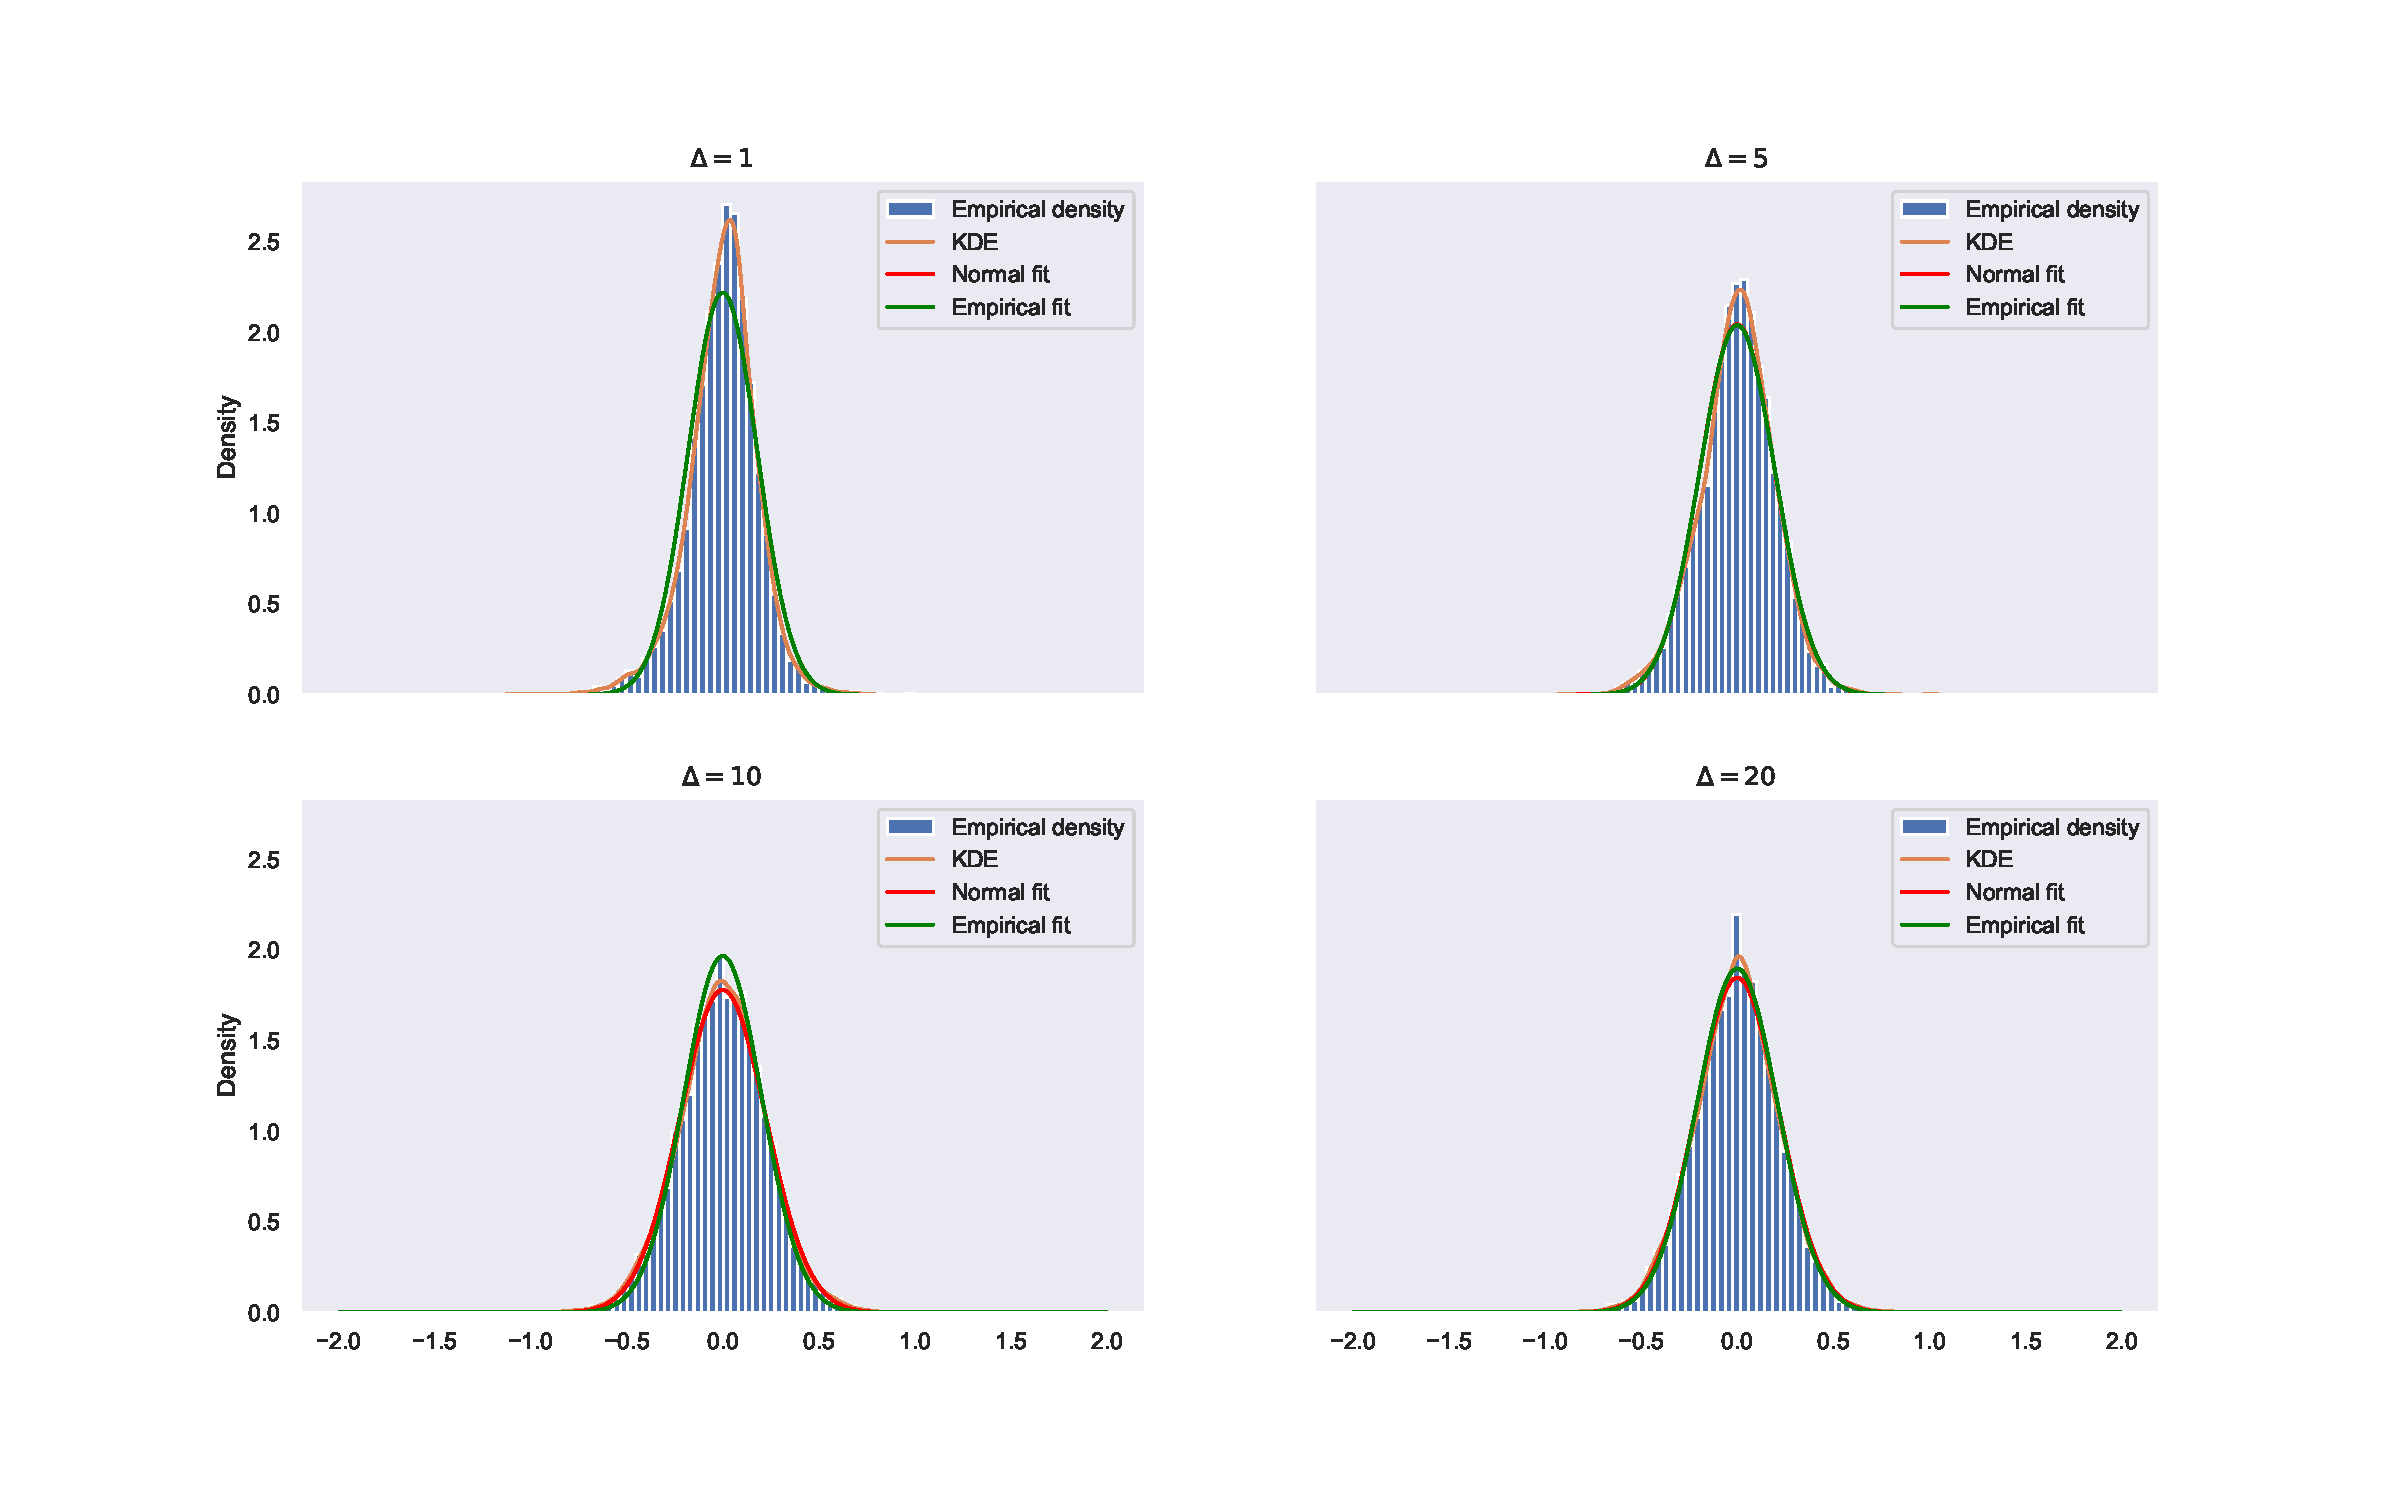
\includegraphics[width=0.7\textwidth]{fig/YNDX RX Equity 30 Lag Hists.pdf}
                    \caption{YNDX RX Equity. Empirical density of $\log \sigma_{t+\Delta} - \log \sigma_{t}$ for $\Delta = 1, 5, 10, 20$ days.}
                    \label{fig:lagHists}
                \end{figure}
            \end{frame}

            \begin{frame}{Visual analysis of histograms and excessed kurtosis plot - III}
                \begin{figure}[htbp]
                    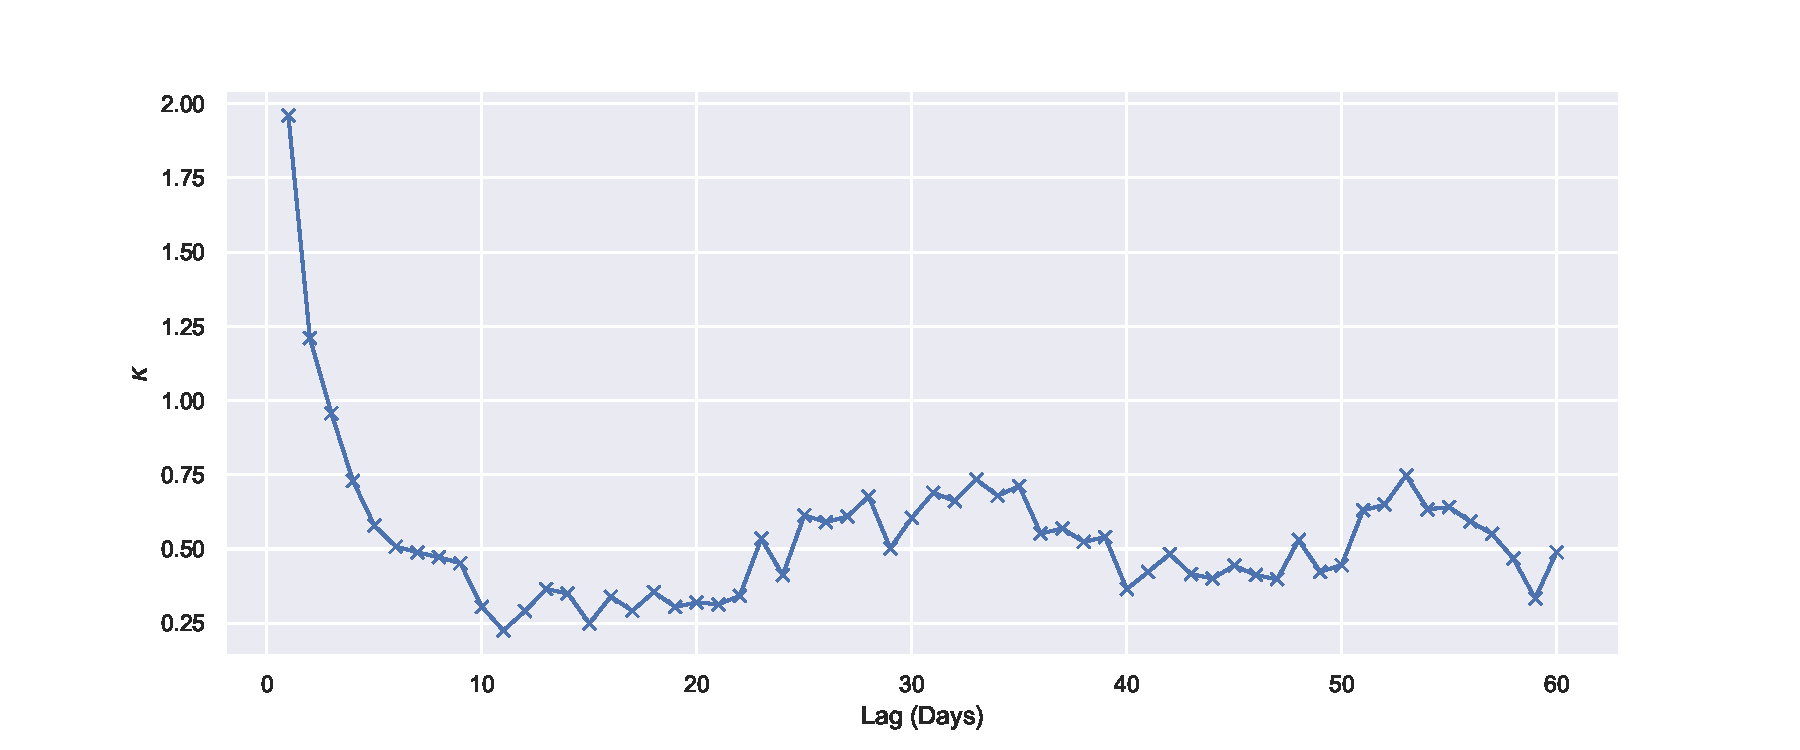
\includegraphics[width=\textwidth]{fig/YNDX RX Equity Excessed Curtosis.pdf}
                    \caption{YNDX RX Equity. Excessed kurtosis $\kappa$ as a function of $\Delta$}
                    \label{fig:exkurt}
                \end{figure}
            \end{frame}

            \begin{frame}{Statistical tests for normality}
                The three possible explanations are:
                \begin{enumerate}
                    \item The tests are correct and the data is not normally distributed or is correlated strongly.
                    \item The visual analysis of the histograms show that for many lags the KDE plot, the normal fit and 
                    the empirical fit are very similar, therefore, the distribution is normal, but the data is 
                    correlated strongly. The excessed kurtosis plot shows that the data is distributed very close to the normal
                    distribution for $\Delta > 5$, and at its closest distance for $\Delta \in [10, 22]$.
                    \item We get a population sampling error (not enough data).
                \end{enumerate} 
            \end{frame}

    \section{Modelless estimator of roughness}
        \subsection{Definitions}
            \begin{frame}{}
                Let us consider a sequence of partitions $\pi^n$ of $\left[0, T\right]$ with 
                $\left|\pi^n\right|:=\max_{t_i^n \in \pi^n} (t_{i+1}^n - t_i^n) \to 0$. 
                \begin{definition}
                    A function $x \in C[0, T]$ is said to have the finite $p$-th variation along the sequence of partitions $\pi^n$ 
                    if there exists a continious increasing function $\left[x\right]_{\pi}^{(p)}$ such that for all subpartitions $\tilde\pi^n(t) = \pi^n \cap [0, t]$
                    \begin{equation}
                        \sum_{t_i^n \in \tilde\pi^n(t)} \left|x(t_{i+1}^n) - x(t_i^n)\right|^p \to \left[x\right]_{\pi}^{(p)}(t), \quad n\to \infty,
                    \end{equation}
                    and the set of all functions having finite $p$-th variation along $\pi$ we denote $V_\pi^p$.
                \end{definition}
            \end{frame}

            \begin{frame}{}
                \begin{definition}
                    The \emph{variation index} of a path $x$ is defined as $p^\pi(x) := \inf \left\{p\geq 1 \colon \quad x\in V_\pi^p\right\}$, and the \emph{roughness index} is defined as $H^\pi(x):=\frac{1}{p^\pi(x)}$.
                \end{definition}
                It has been proven that for fBm with Hurst parameter $H$ 
                
                \noindent $p^\pi(W^H) = \frac{1}{H}$ and $H^\pi(W^H) = H$.
                
                \begin{definition}
                    $x\in V_\pi^p$ is said to have $p$-th normalized variation if there exists such continious function $w(x, p, \pi)\colon [0, T] \to \mathbb{R}$ that
                    \begin{equation}
                        \sum_{\tilde\pi^n(t)}\frac{\left|x(t_{i+1}^n) - x(t_i^n)\right|^p}{\left[x\right]_{\pi}^{(p)}(t_{i+1}^n)-\left[x\right]_{\pi}^{(p)}(t_i^n)} (t_{i+1}^n-t_{i}^n) \to w(x, p, \pi).
                    \end{equation}
                \end{definition}
            \end{frame}

            \begin{frame}{}
                Let us consider $\pi^L$, $\pi^K$ -- partitions with sampling frequencies $L\gg K$ ($\pi^K \subset \pi^L$).
                \begin{definition}
                    Sample normalized $p$-th variation is defined as
                    \begin{equation}
                        W(L, K, p, t, X) = \sum_{\tilde\pi^K(t)}\frac{\left|x(t_{i+1}^K) - x(t_i^K)\right|^p}{\sum_{t_i^n \in \tilde\pi^n(t)} \left|x(t_{i+1}^n) - x(t_i^n)\right|^p} (t_{i+1}^n-t_{i}^n)
                    \end{equation}
                \end{definition}
                It has been proven that\begin{itemize}
                    \item $W$ converges to $w$ as sampling frequencies tend to $\infty$;
                    \item $W$ is strictly monotonic in $p$.
                \end{itemize}
                This method was introduced in [CD22].
            \end{frame}
            
            \begin{frame}{}
                \begin{figure}[htbp]
                    \centering
                    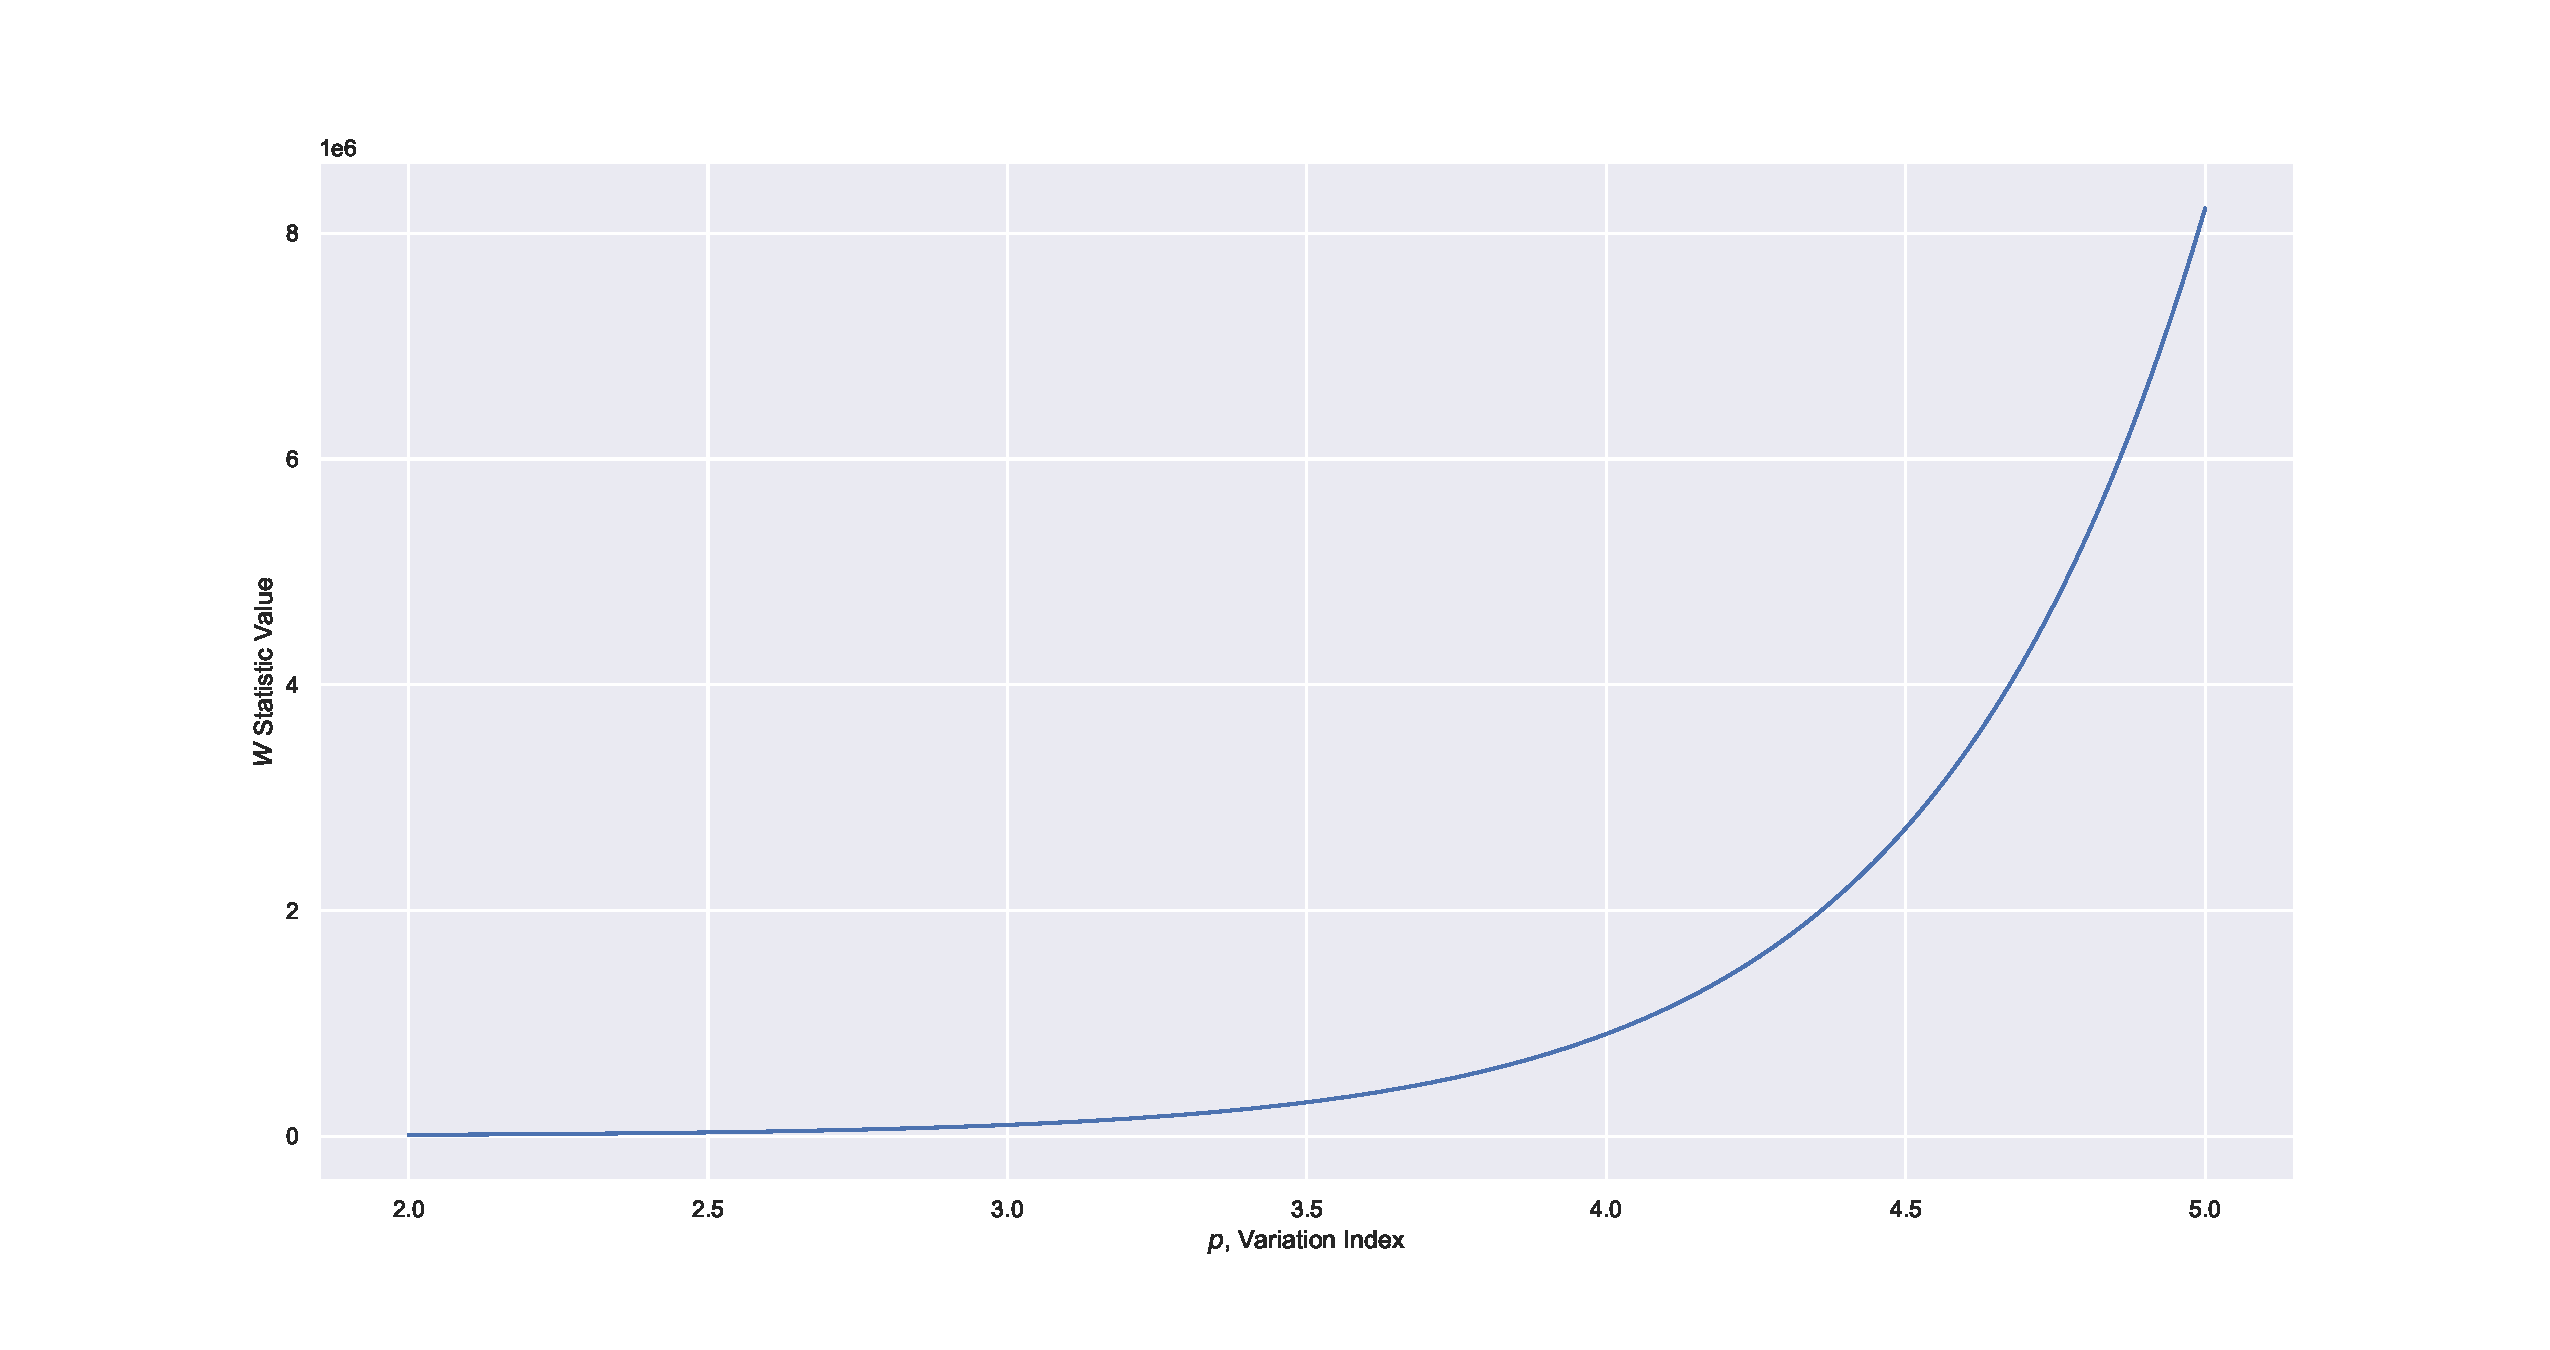
\includegraphics[width=0.9\linewidth]{fig/W Stat Illustration.pdf}
                    \caption{The $W$ statistic as a function of $p$}
                \end{figure}
            \end{frame}

        \subsection{Roughness estimation of Monte-Carlo simulations of fBm}
            \begin{frame}{}
                \begin{figure}[htbp]
                    \centering
                    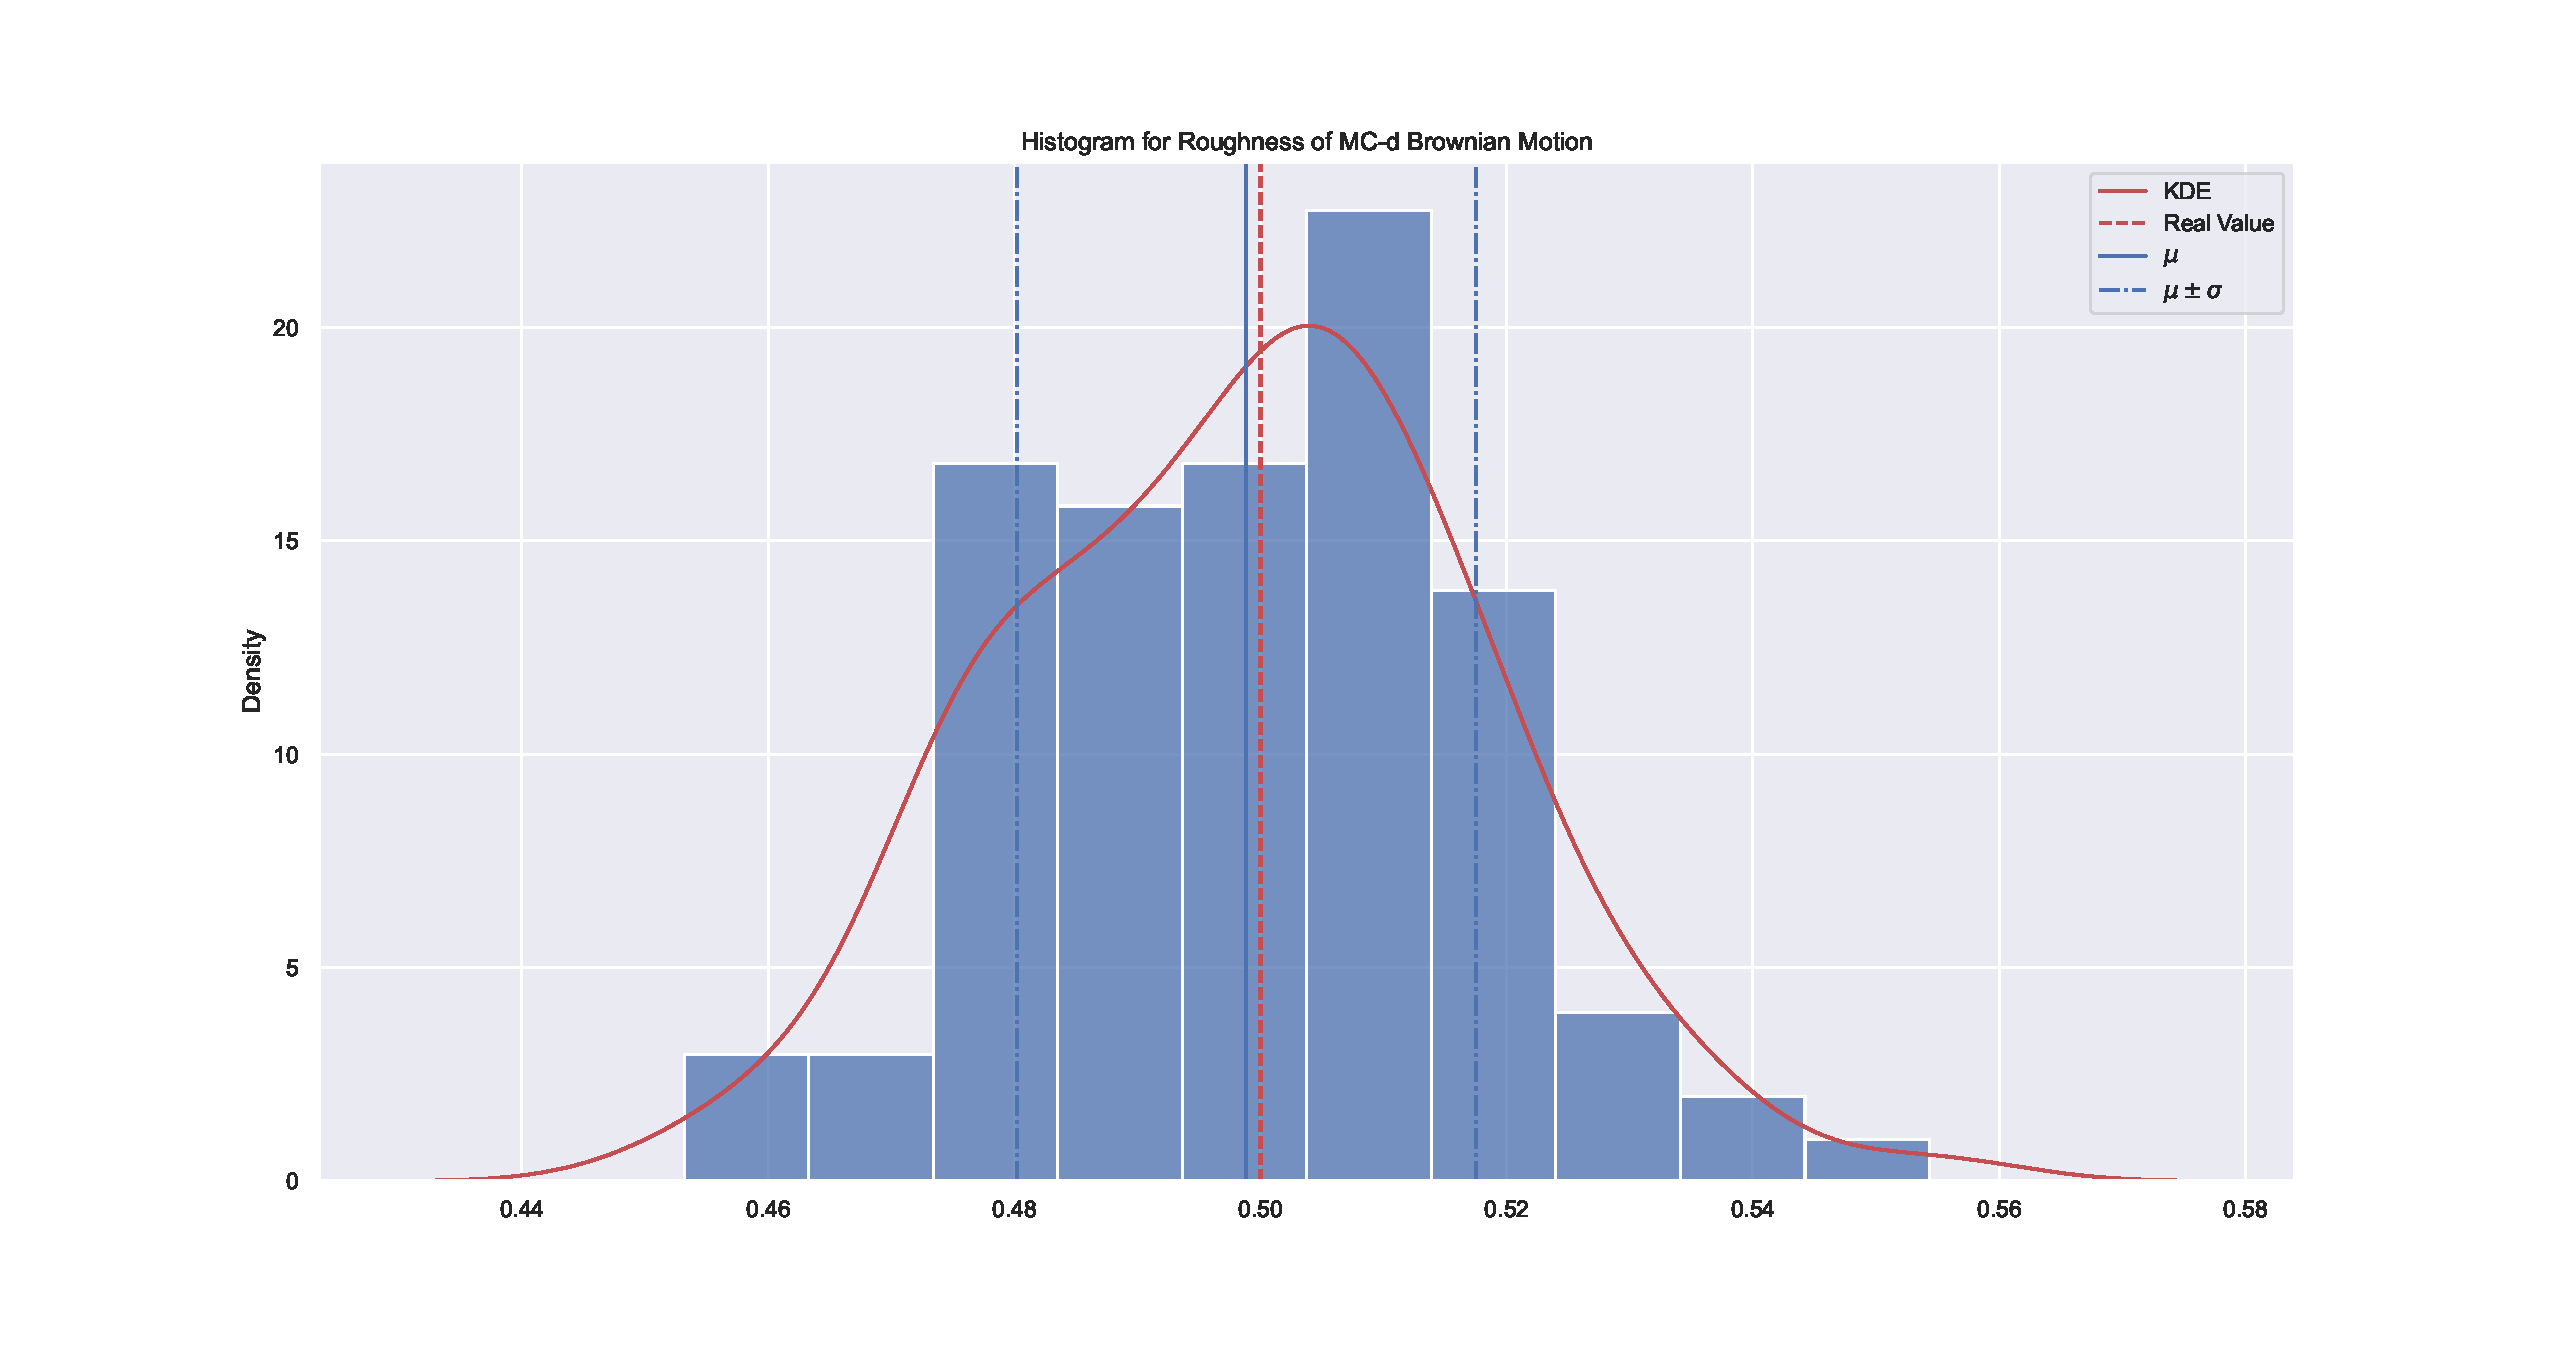
\includegraphics[width=0.9\linewidth]{fig/Histogram for Roughness of MC-d Brownian Motion.pdf}
                    \caption{Histogram for roughness of Brownian motion, $\hat H = 0.4988$}
                \end{figure}
            \end{frame}

            \begin{frame}{}
                \begin{figure}[htbp]
                    \centering
                    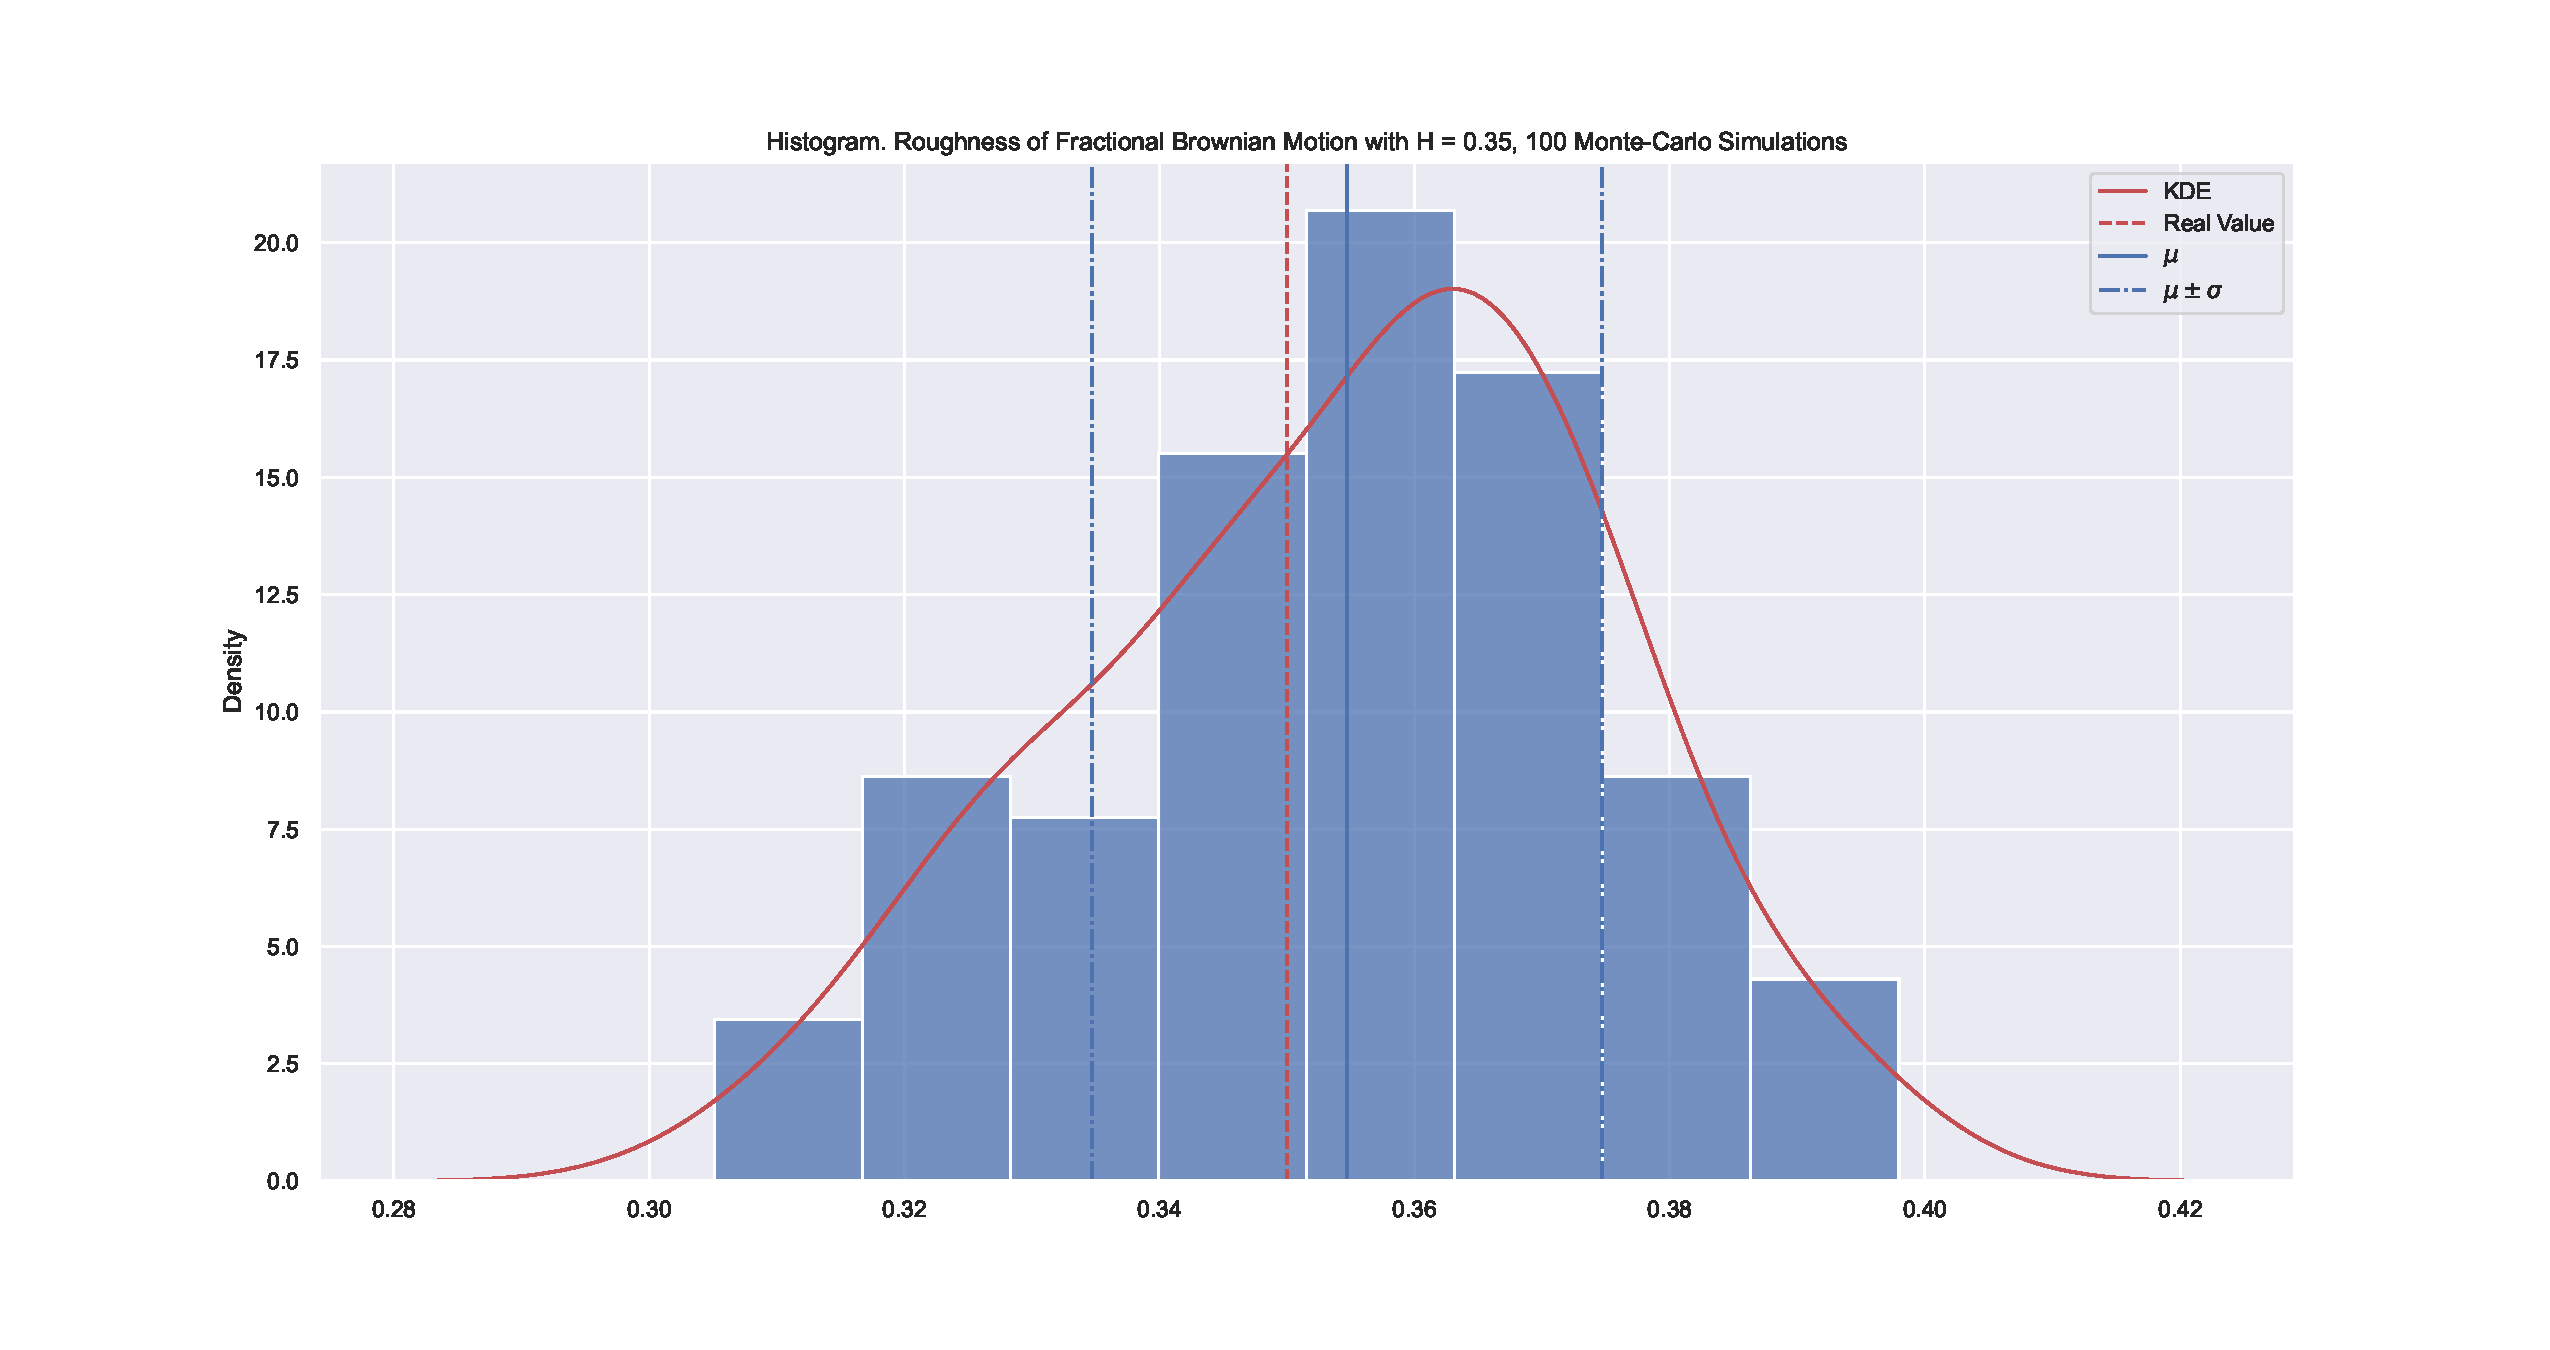
\includegraphics[width=0.9\linewidth]{fig/Histogram. Roughness of Fractional Brownian Motion with H = 0.35, 100 Monte-Carlo Simulations.pdf}
                    \caption{Histogram for roughness of fractional Brownian motion, $H = 0.35$, $\hat{H} = 0.3547$}
                \end{figure}
            \end{frame}
            
            \begin{frame}{}
                \begin{figure}[htbp]
                    \centering
                    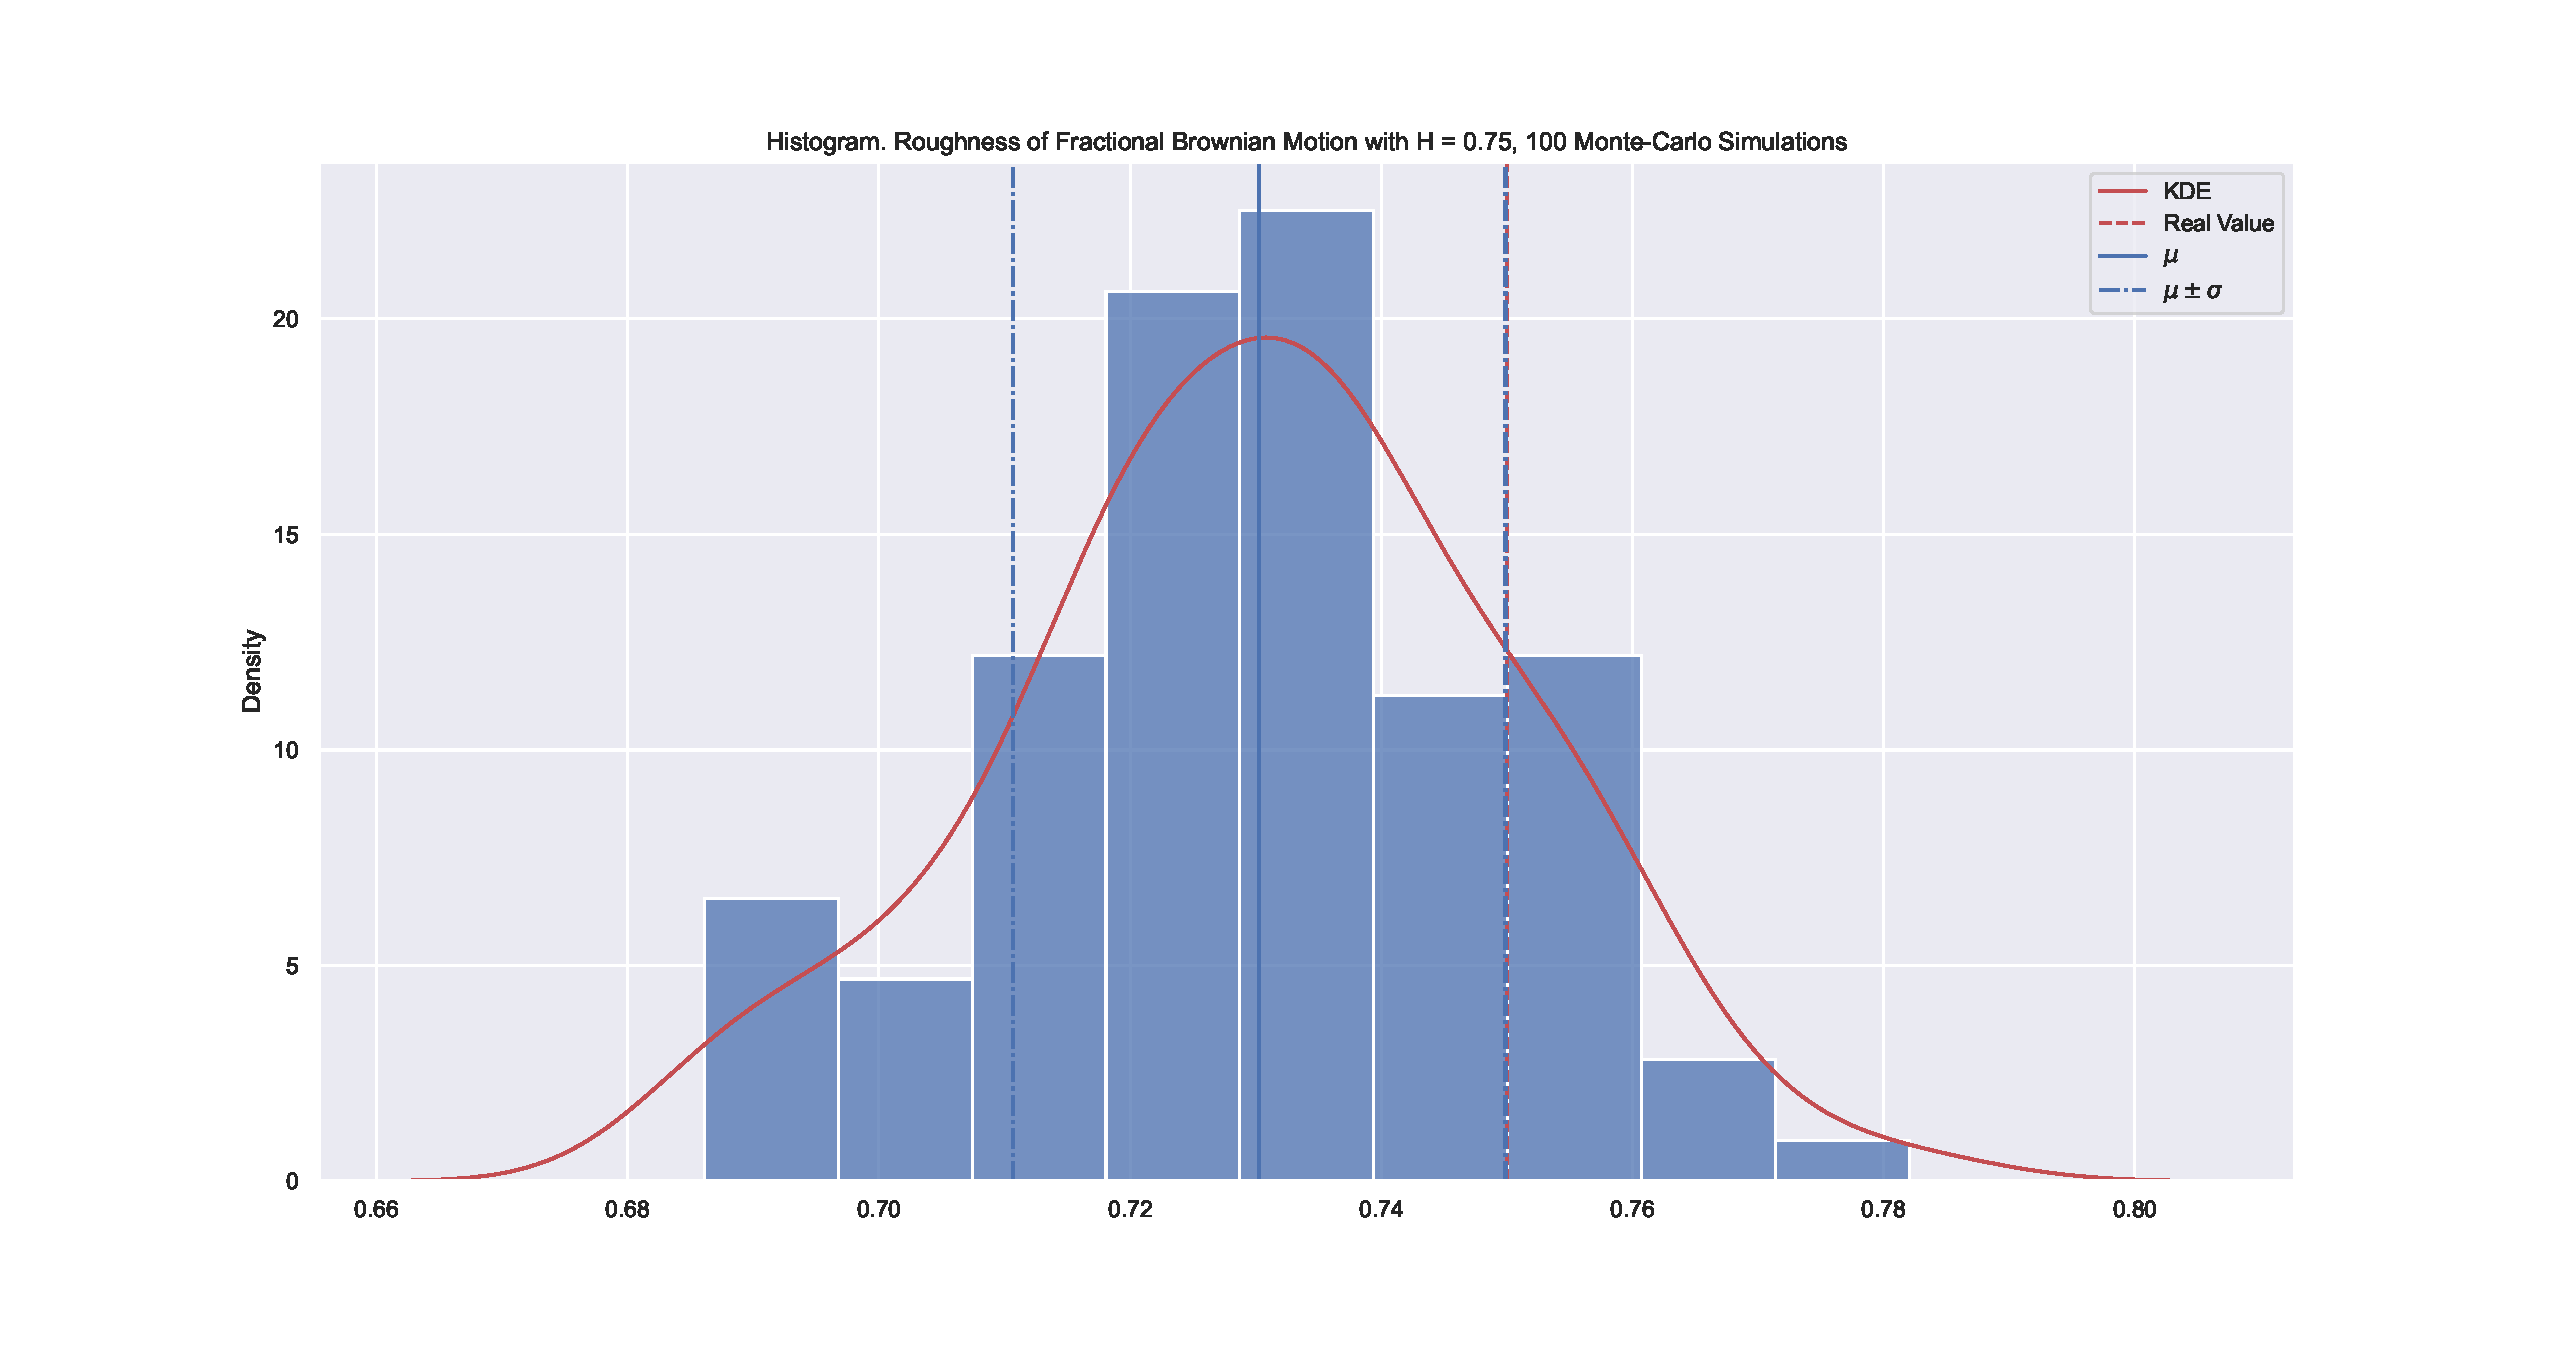
\includegraphics[width=0.9\linewidth]{fig/Histogram. Roughness of Fractional Brownian Motion with H = 0.75, 100 Monte-Carlo Simulations.pdf}
                    \caption{Histogram for roughness of fractional Brownian motion, $H = 0.35$, $\hat{H} = 0.7302$}
                \end{figure}
            \end{frame}
        \subsection{Roughness estimation of Monte-Carlo simulations of Heston stochastic volatility model}
            \begin{frame}{}
                \begin{figure}[htbp]
                    \centering
                    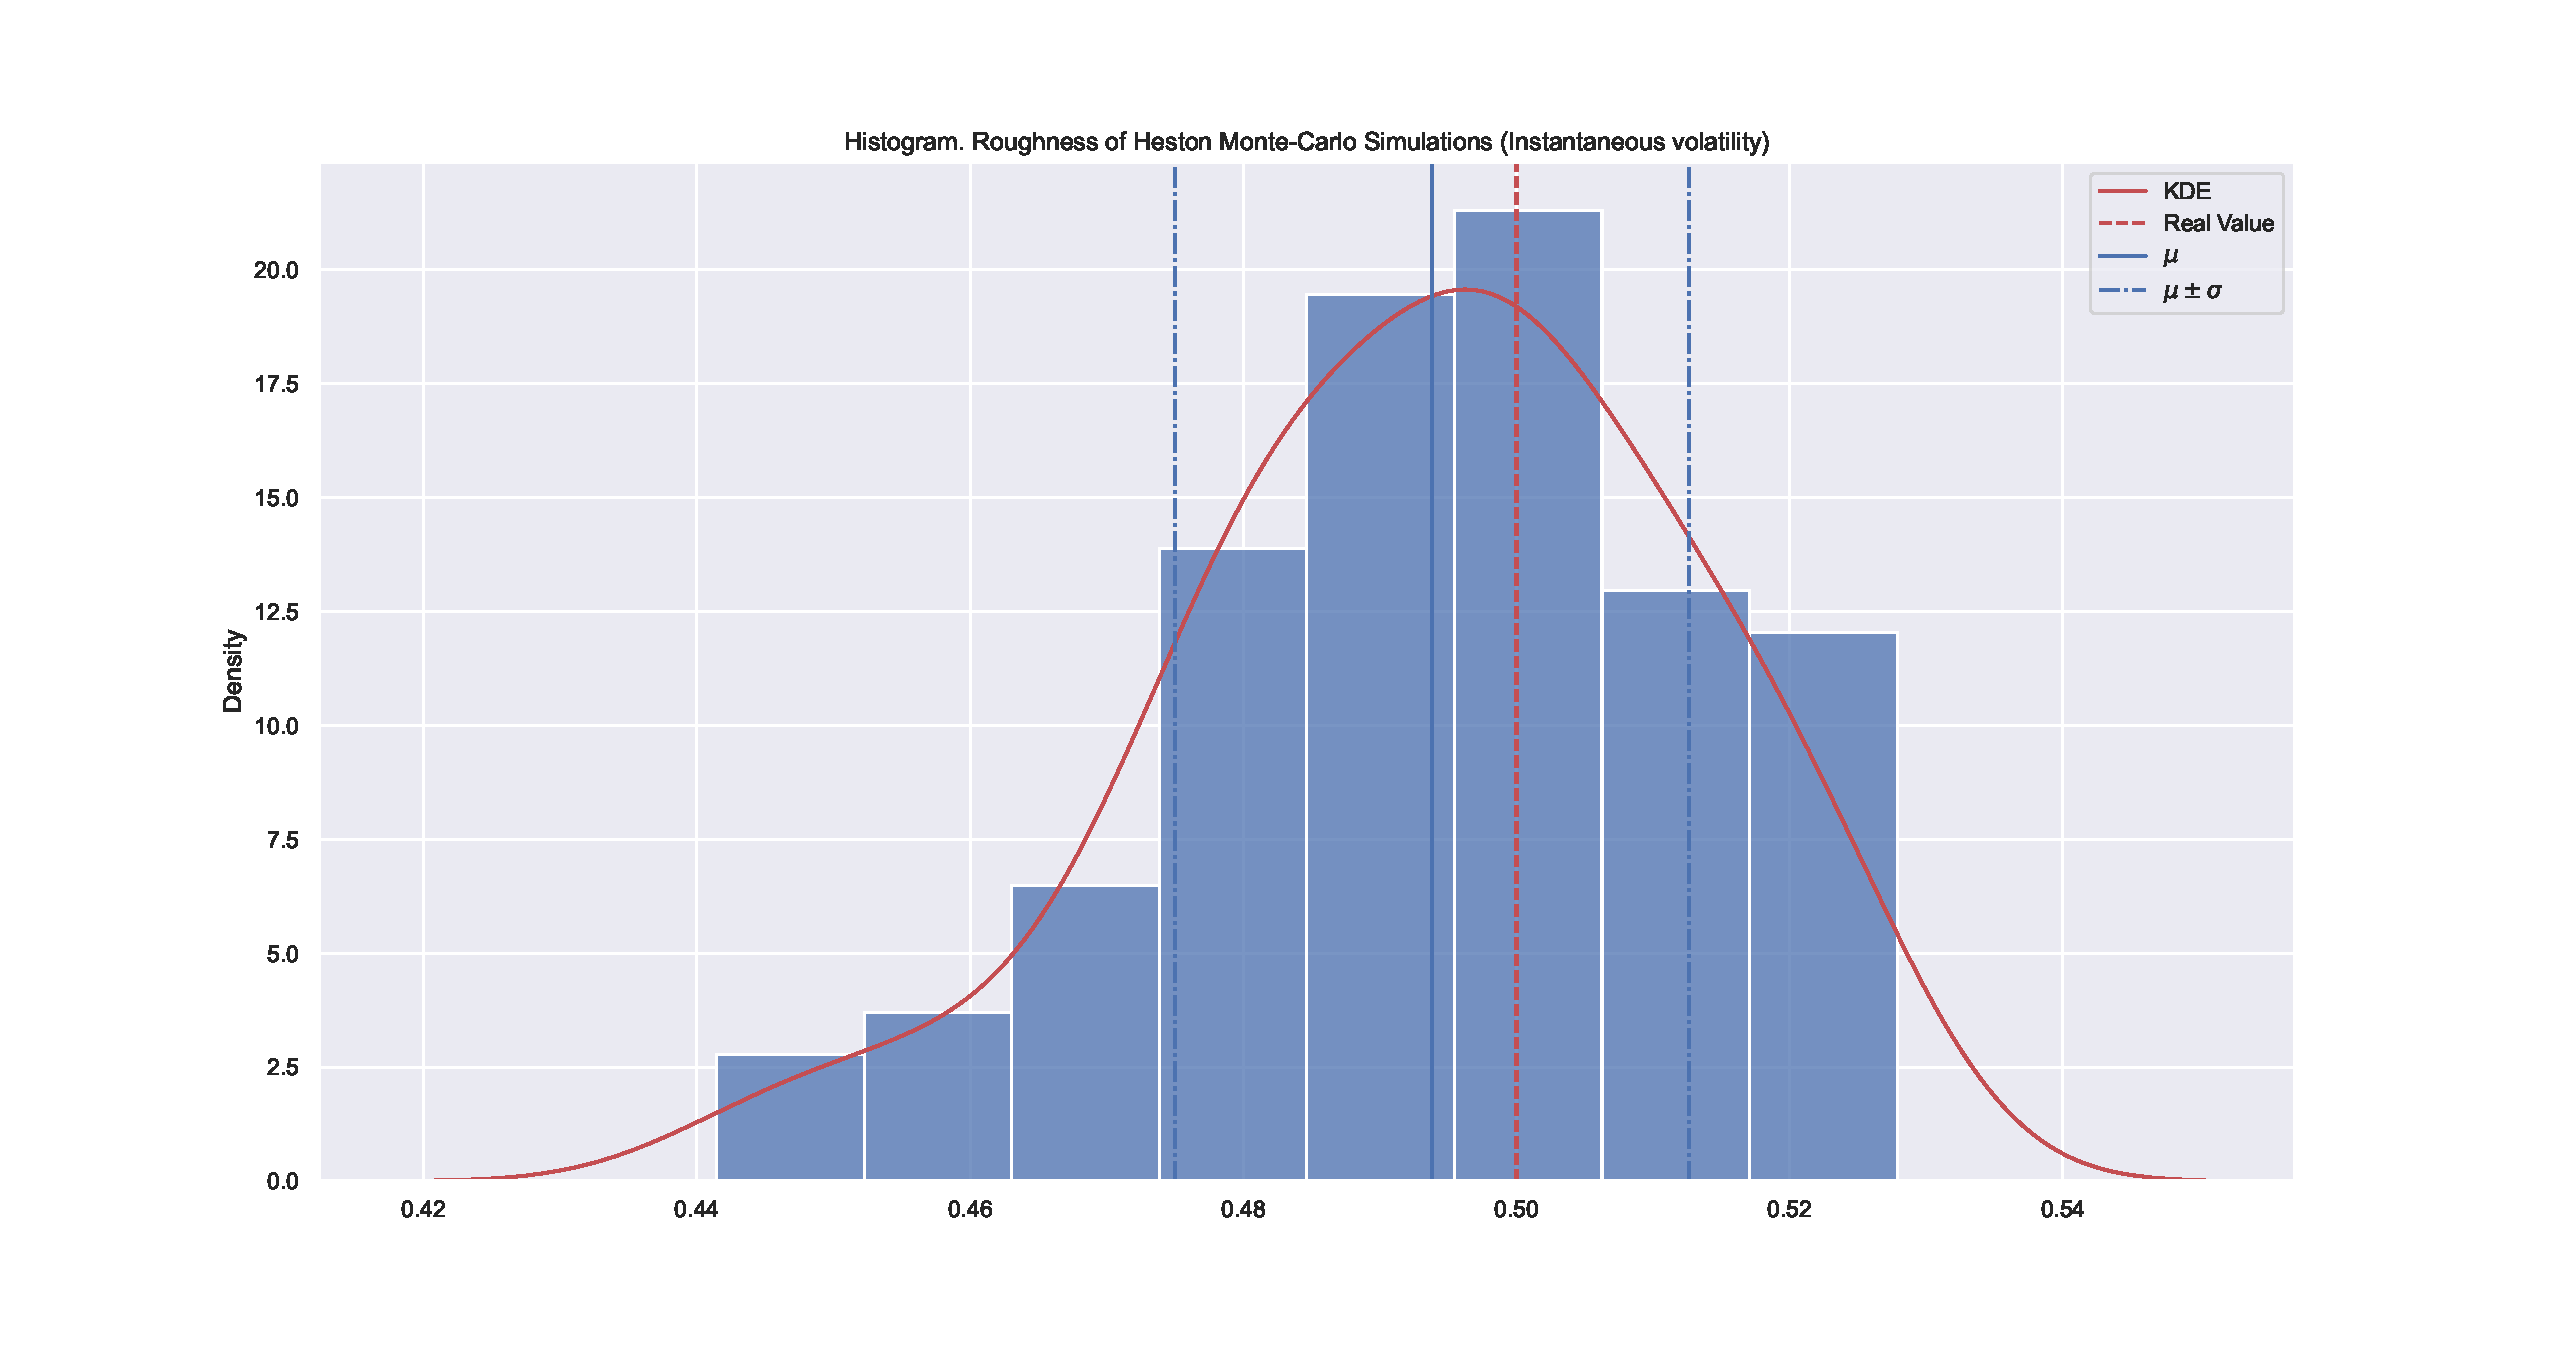
\includegraphics[width=0.9\linewidth]{fig/Histogram. Roughness of Heston Monte-Carlo Simulations (Instantaneous volatility).pdf}
                    \caption{Histogram for roughness of Heston SVM (Instantaneous volatility)}
                \end{figure}
            \end{frame}

            \begin{frame}{}
                \begin{figure}[htbp]
                    \centering
                    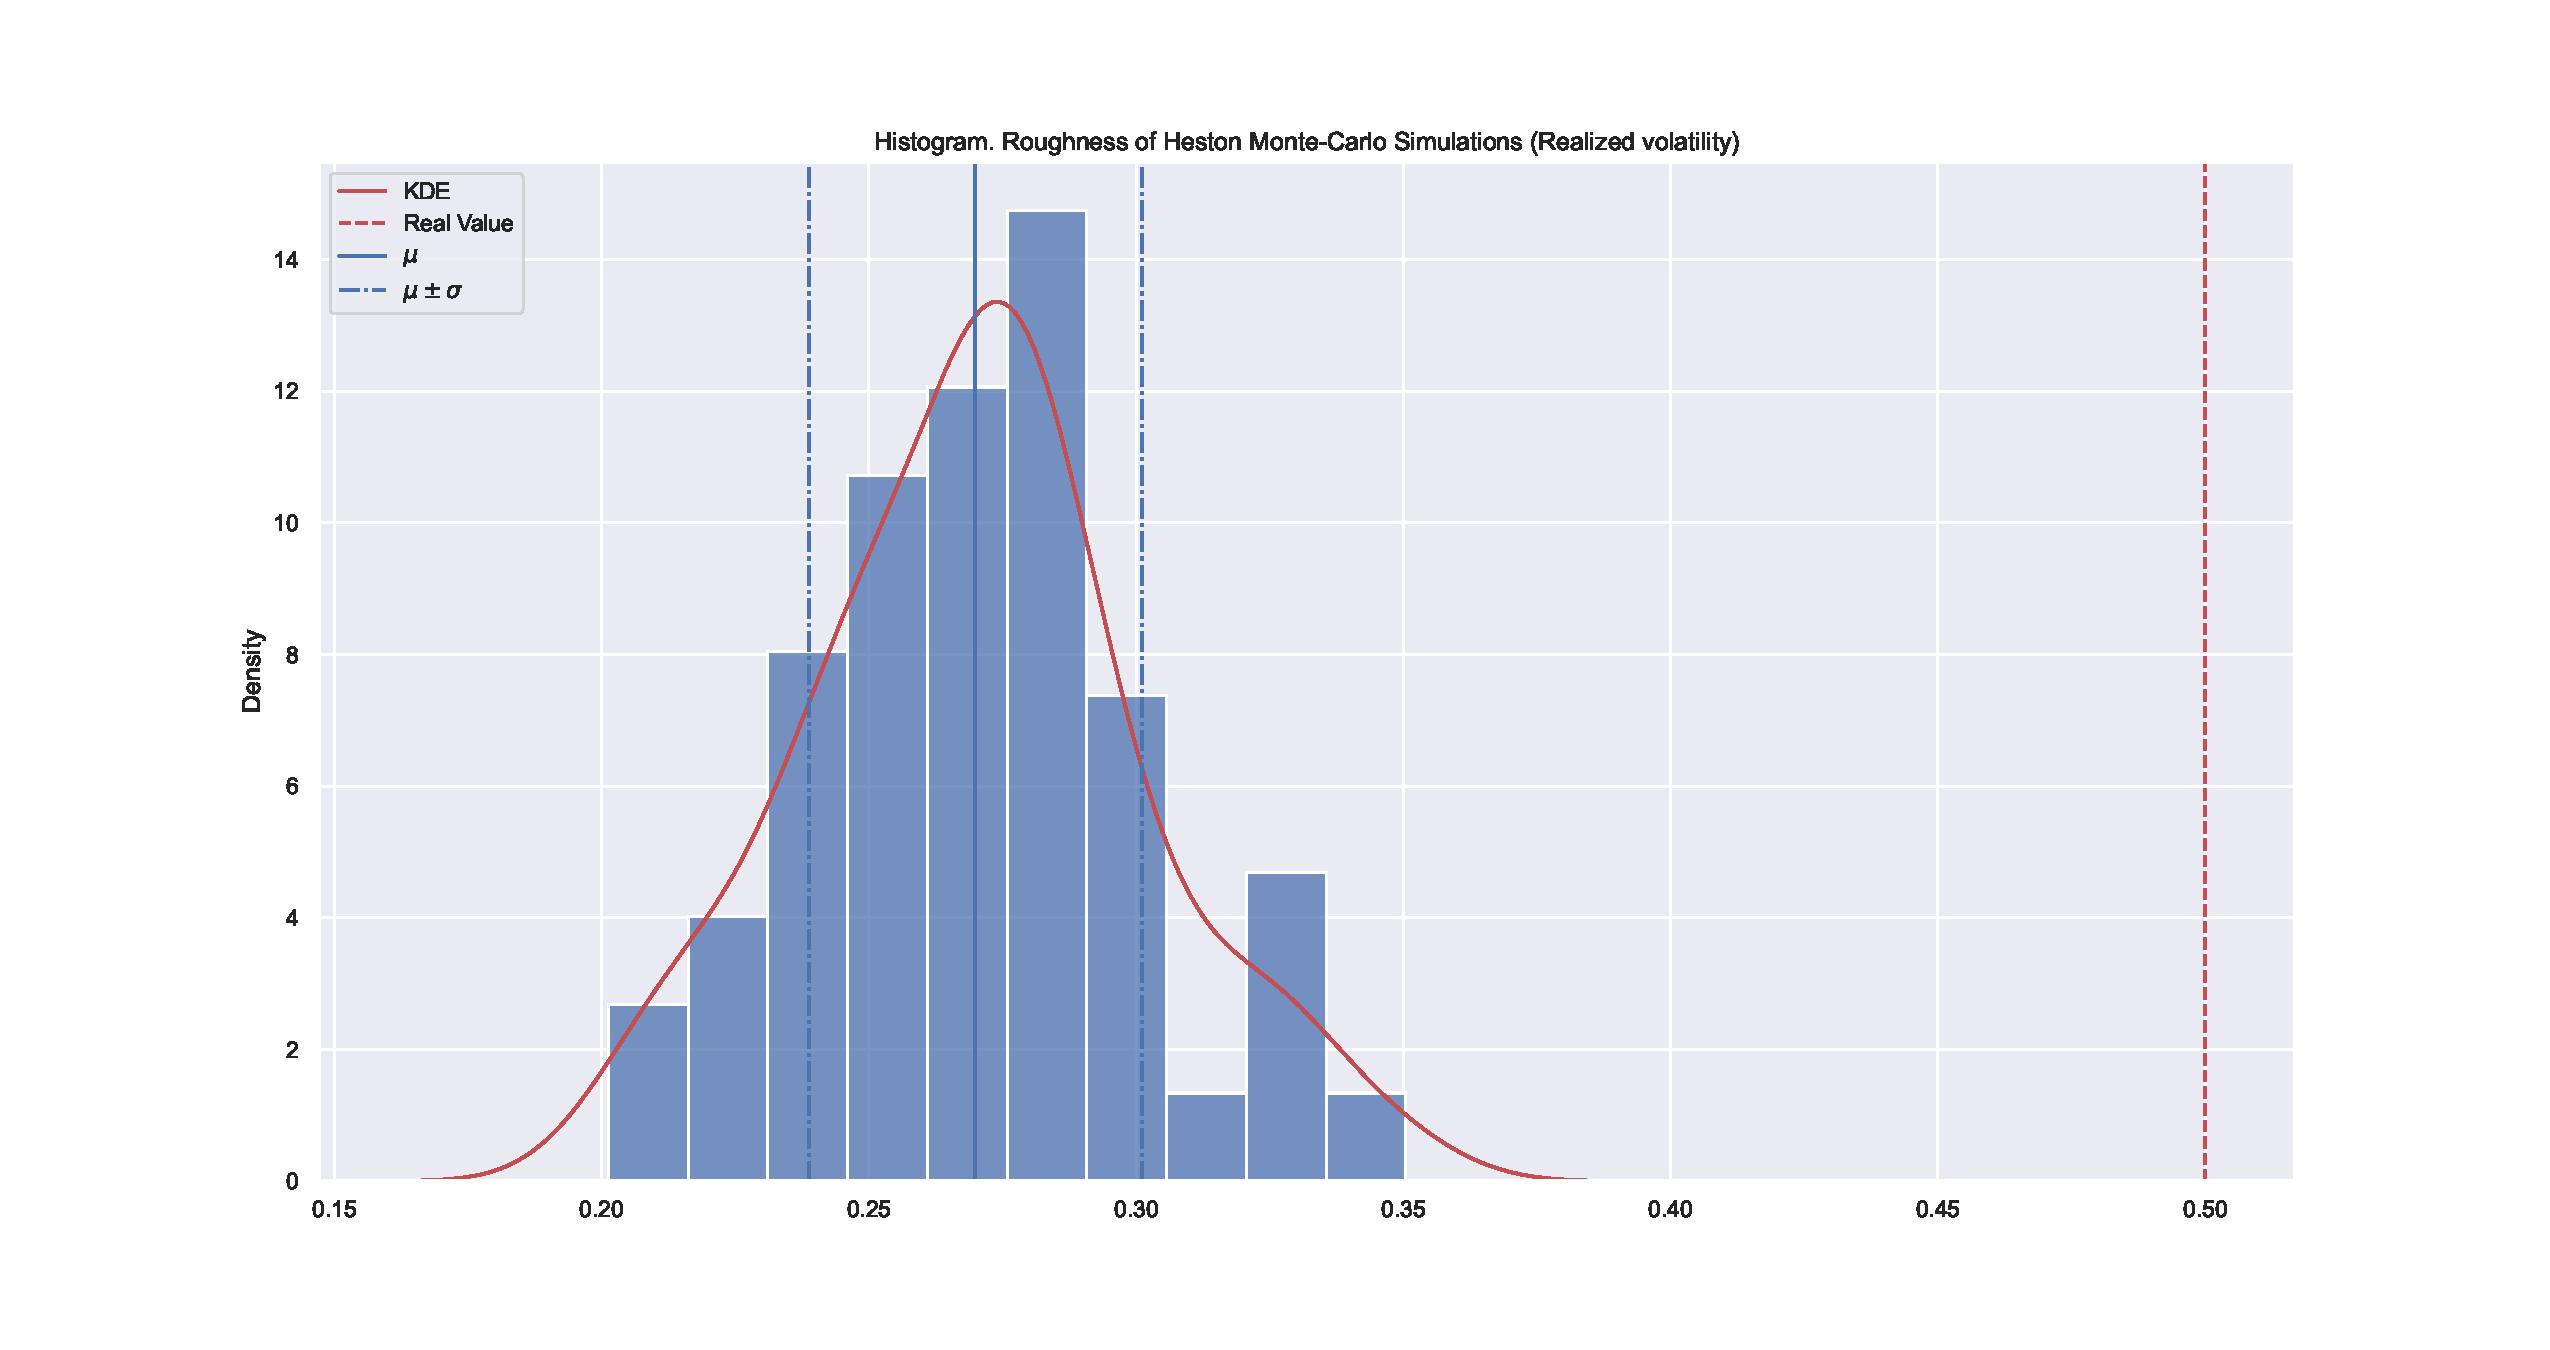
\includegraphics[width=0.9\linewidth]{fig/Histogram. Roughness of Heston Monte-Carlo Simulations (Realized volatility).pdf}
                    \caption{Histogram for roughness of Heston SVM (Realized volatility)}
                \end{figure}
            \end{frame}

        \subsection{Roughness estimation of real market data}
            \begin{frame}
                \begin{table}[h]
                    \centering
                    \begin{tabular}{|c|c|c|c|c|c|}
                        \hline
                        Ticker &  Roughness Index\\\hline
                        \hline
                        YNDX RX Equity & 0.372691\\\hline
                        SBER RX Equity & 0.313109\\\hline
                        VTBR RX Equity & 0.304677\\\hline
                        MOEX RX Equity & 0.295378\\\hline
                        LKOH RX Equity & 0.301795\\\hline
                        GAZP RX Equity & 0.316125\\\hline
                        FIVE RX Equity & 0.284704\\\hline
                        \hline
                        OGZD LI Equity & \alert{2.968608}\\\hline
                        VTBR LI Equity & 0.306763\\\hline
                        SBER LI Equity & \alert{1.176616}\\\hline
                        LKOD LI Equity & 0.306061\\\hline
                    \end{tabular}
                    \caption{Roughness index estimation}
                    \label{tab:roughness_index}
                \end{table}
            \end{frame}

        \section*{Bibliography}
            \begin{frame}{Base articles}
                \begin{itemize}
                    \item[GJR14] Jim Gatheral, Thibault Jaisson, and Mathieu Rosenbaum. “Volatility is rough”. In: \emph{Quantitative Finance} 18.6 (2014), pp. 933–949;
                    \item[Ros08] Mathieu Rosenbaum. “Estimation of the volatility persistence in a discretely observed diffusion model”. In: \emph{Stochastic Processes and their Applications} 118.8 (2008), pp. 1434–1462;
                    \item[CD22]  Rama Cont and Purba Das. “Rough volatility: fact or artefact?” In: (2022).
                \end{itemize}
            \end{frame}
\end{document}